\clearpage

\section{Binning studies}
\label{appendix:mc_template_binning_studies}

%
% ----------------------------------------
%

% Text

\subsection{True energy binning}
\label{appendix:mc_template_binning_studies:etrue}

The chosen true neutrino energy binning scheme needs to have enough granularity for precise application of oscillation
probabilities and of systematic parameter response functions (with the former proven to be the primary consideration).
The chosen 84-bin scheme is described in Section \ref{sec:mc_templates:template_binning}. 
This binning scheme was selected as a trade-off between CPU efficiency and accuracy,
as oscillation probabilities are calculated at the centre of each true energy bin.
Single $\mu$-like ring event reconstructed energy spectra obtained with the chosen binning scheme
were compared against spectra obtained with an alternative, much finer, binning scheme.
The alternative scheme uses 780 bins as follows:
200 5-MeV bins in 0-1 GeV and 580 50-MeV bins in 1-30 GeV.
Figs.\ \ref{fig:etruebin:numuccqe}-\ref{fig:etruebin:signueccoth} show the ratio of indiviual SuperK MC mode $E_{reco}$ spectra, made with 84-bin $E_{true}$ and 780-bin $E_{true}$.
While there are some $>$1\% differences, these occur in modes that are a small contribution to the total $E_{reco}$ spectrum.
This is reiterated in Fig.\ \ref{fig:etruebin:total}, which shows the same ratio, but for the total $E_{reco}$ spectrum.

% ..

\subsection{Reconstructed energy binning}
\label{appendix:mc_template_binning_studies:ereco}

The chosen reconstructed neutrino energy binning scheme needs to have sufficient granularity 
(considering the experimental reconstructed neutrino energy resolution and the current statistics)
to allow a precise determination of neutrino oscillation parameters while, at the same time,
a reasonable CPU efficiency is retained.
The binning also needs to be fine enough to allow the precise application of systematic parameter response functions
in the p.d.f. (discussed in Appendix \ref{appendix:mc_template_binning_studies:spline}).
The selected reconstructed neutrino energy binning scheme (73 bins) is shown in Appendix \ref{sec:mc_templates:template_binning}.
A sensitivity study (see Appendix \ref{appendix:sensitivity_study} for details) at the MINOS 2012 best fit point
has been performed with an alternative, much finer, reconstructed energy binning scheme: 600 50 MeV bins, 0 - 30 GeV.
The result can be seen in Fig. \ref{fig:apdx:bin:sensitivity:600vs73}.
The plot shows that the chosen 73-bin scheme is sufficient.

% ..

\subsection{SuperK MC templates in the chosen binning}
\label{appendix:mc_template_binning_studies:templates}

The nominal SuperK MC templates, in the chosen binning, are shown 
in Figs. \ref{fig:etrue_ereco_templates:numu}-\ref{fig:etrue_ereco_templates:signue}.

% ..

\subsection{True and reconstructed energy binning for systematic parameter response functions}
\label{appendix:mc_template_binning_studies:spline} 

Systematic parameter response functions (cubic splines) were constructed in bins of true and reconstructed energy.
This binning is given in Sec.\ \ref{sec:systematics:inputs:uncor_xsec}.
A study was performed to check the effect of this binning.
This was done by creating tweaked single $\mu$-like ring event reconstructed energy spectra using the splines, and comparing them with 
the equivalent tweaked spectra made with event-by-event reweighting (the latter being too CPU-demanding to be used in the oscillation parameter fit). 
Both the spline spectra and the event-by-event spectra were made for no oscillations.
The 73-bin scheme for the Monte Carlo templates given in Sec.\ \ref{sec:mc_templates:template_binning} was used. 
Some examples of the ratios of the 
spline spectra to the event-by-event reweighted spectra are shown in Figs.\ \ref{fig:spline_binning_studies:maqe}-\ref{fig:spline_binning_studies:ccothershape}. 
They show that the ratios are very close to 1.0 for the $\nu_{\mu}$ and $\bar{\nu}_{\mu}$ spectra,
which comprise the bulk of the total predicted single $\mu$-like ring spectrum. 


%
% ----------------------------------------
%

%
% Figs for \subsection{$E_{true}$ binning}
%

\begin{figure*}[htb]
\begin{minipage}[t]{0.48\linewidth}
\center
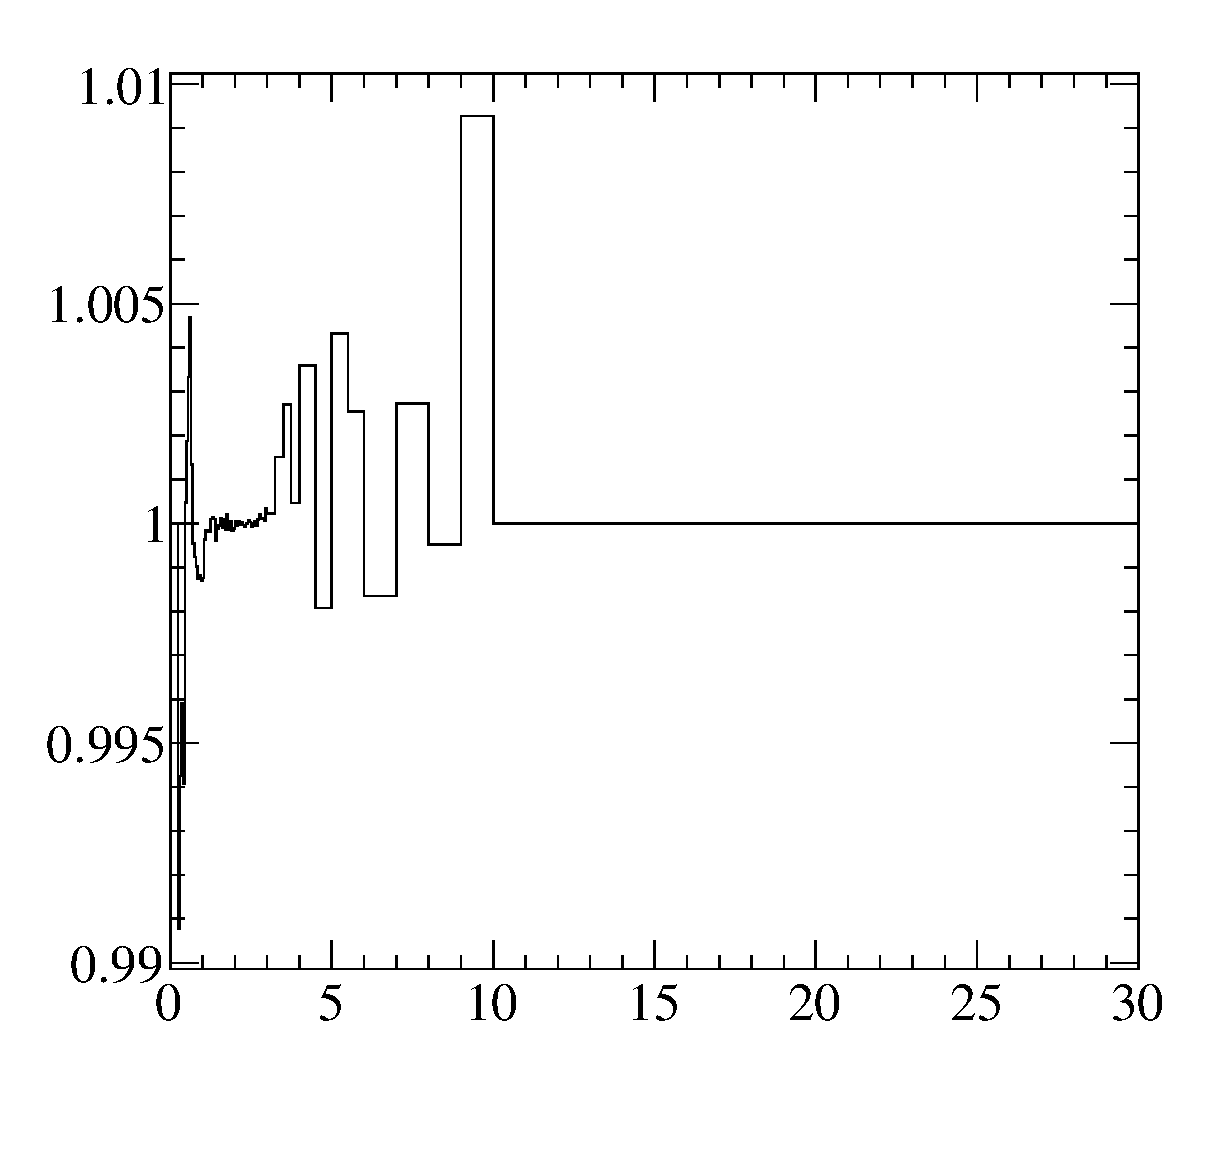
\includegraphics[width=18pc]{./images/binning/oscillation/plot_erec_int_numu_ccqe_fine}
\caption
 {Ratio of SuperK MC $E_{reco}$ spectra, for mode $\nu_\mu$ CCQE made with 84 bin $E_{true}$ and 780 bin $E_{true}$, for an exposure of 3.010$	imes$10$^{20}$ POT. The number of events was calculated using the BANFF-tuned MC templates.Using oscillation parameters:  $\sin^22\theta_{12} = $0.857; $\sin^22\theta_{13} = $0.098; $\sin^22\theta_{23} = $1; $\delta_{CP} = $        0; $\Delta m^2_{21} = $    7.5e-05 $eV^2/c^4$; $|\Delta m^2_{32}| = $    0.0024 $eV^2/c^4$. }
\label{fig:etruebin:numuccqe}
\end{minipage}
\hspace{0.06\linewidth}
\begin{minipage}[t]{0.48\linewidth}
\center
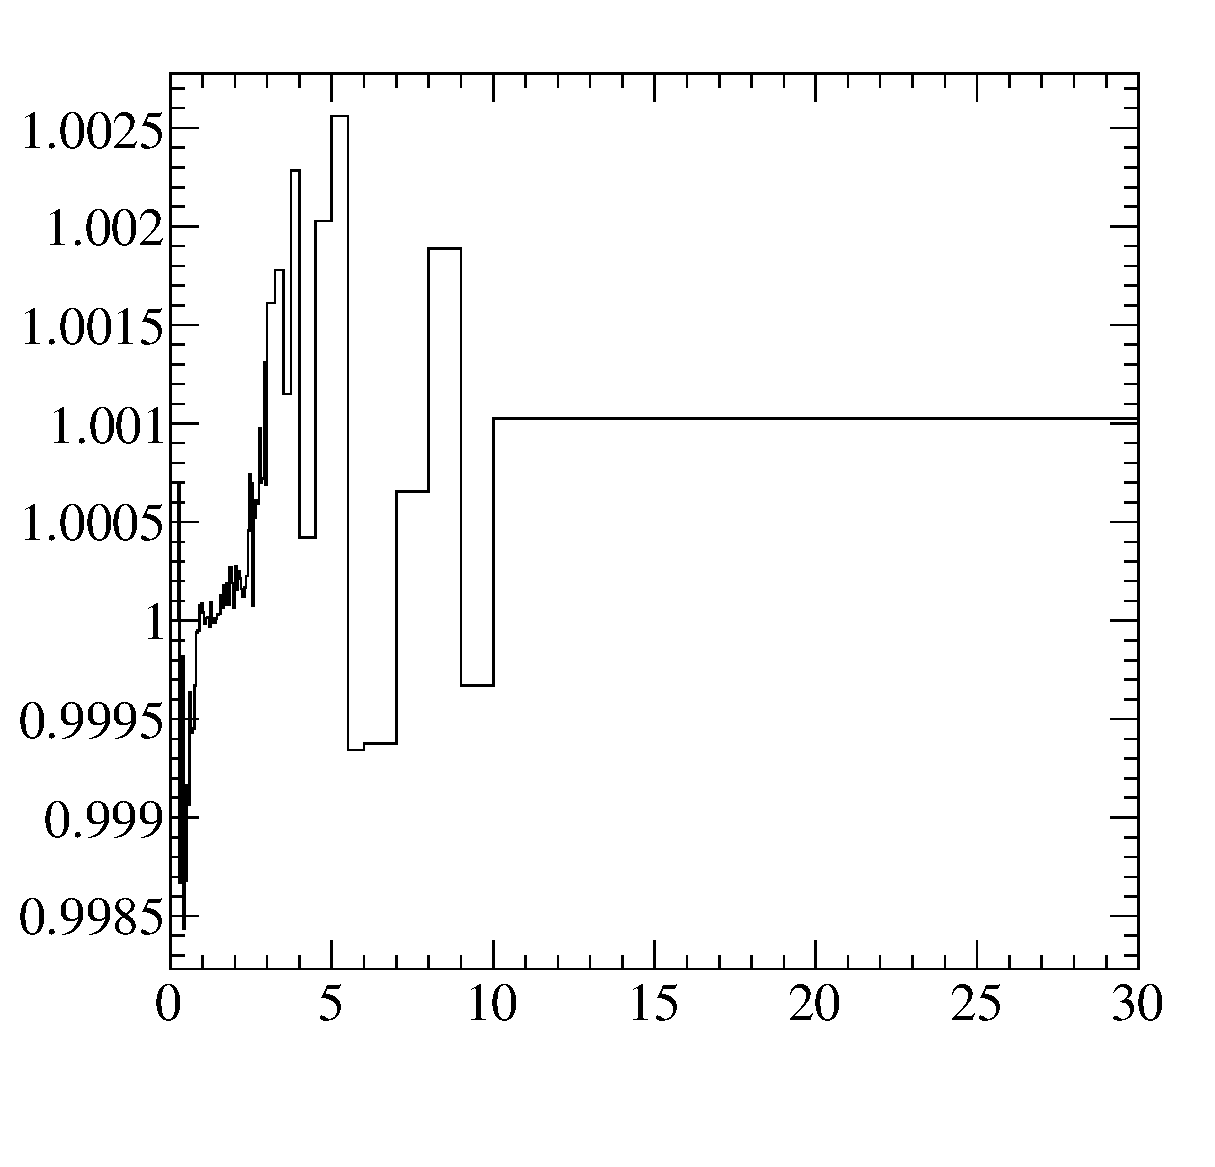
\includegraphics[width=18pc]{./images/binning/oscillation/plot_erec_int_numu_ccpi_fine}
\caption
 {Ratio of SuperK MC $E_{reco}$ spectra, for mode $\nu_\mu$ CC 1$\pi$ made with 84 bin $E_{true}$ and 780 bin $E_{true}$, for an exposure of 3.010$	imes$10$^{20}$ POT. The number of events was calculated using the BANFF-tuned MC templates.Using oscillation parameters:  $\sin^22\theta_{12} = $0.857; $\sin^22\theta_{13} = $0.098; $\sin^22\theta_{23} = $1; $\delta_{CP} = $        0; $\Delta m^2_{21} = $    7.5e-05 $eV^2/c^4$; $|\Delta m^2_{32}| = $    0.0024 $eV^2/c^4$. }
\label{fig:etruebin:numucc1pi}
\end{minipage}
\vfill
\begin{minipage}[t]{0.48\linewidth}
\center
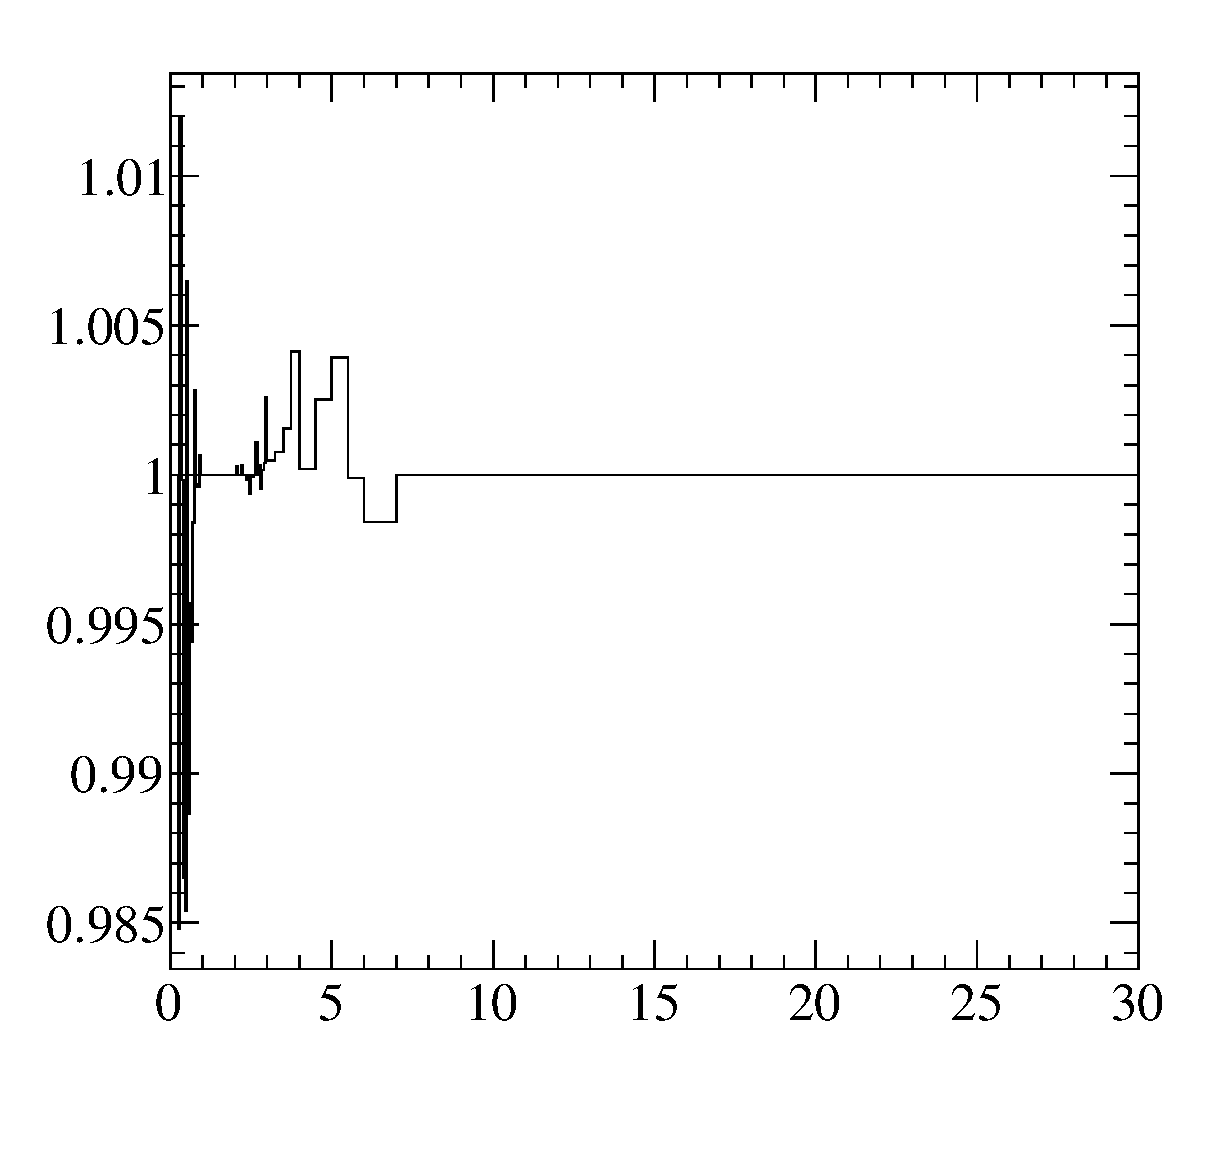
\includegraphics[width=18pc]{./images/binning/oscillation/plot_erec_int_numu_cccoh_fine}
\caption
 {Ratio of SuperK MC $E_{reco}$ spectra, for mode $\nu_\mu$ CC coherent made with 84 bin $E_{true}$ and 780 bin $E_{true}$, for an exposure of 3.010$	imes$10$^{20}$ POT. The number of events was calculated using the BANFF-tuned MC templates.Using oscillation parameters:  $\sin^22\theta_{12} = $0.857; $\sin^22\theta_{13} = $0.098; $\sin^22\theta_{23} = $1; $\delta_{CP} = $        0; $\Delta m^2_{21} = $    7.5e-05 $eV^2/c^4$; $|\Delta m^2_{32}| = $    0.0024 $eV^2/c^4$. }
\label{fig:etruebin:numucccoh}
\end{minipage}
\hspace{0.06\linewidth}
\begin{minipage}[t]{0.48\linewidth}
\center
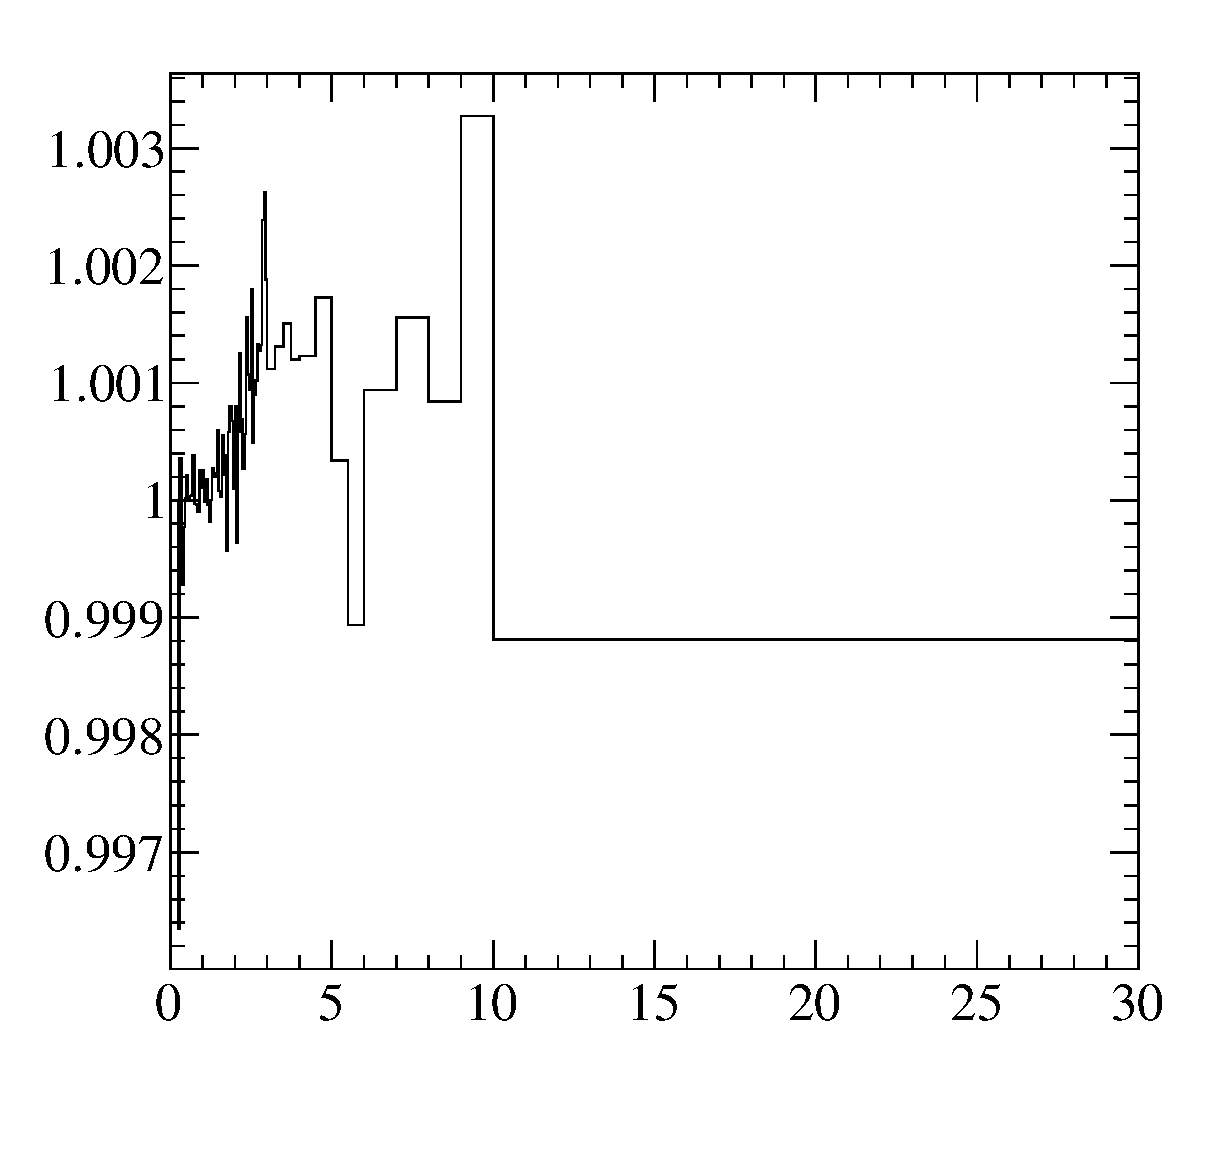
\includegraphics[width=18pc]{./images/binning/oscillation/plot_erec_int_numu_ccoth_fine}
\caption
 {Ratio of SuperK MC $E_{reco}$ spectra, for mode $\nu_\mu$ CC other ($\nu_\mu$ disap) made with 84 bin $E_{true}$ and 780 bin $E_{true}$, for an exposure of 3.010$	imes$10$^{20}$ POT. The number of events was calculated using the BANFF-tuned MC templates.Using oscillation parameters:  $\sin^22\theta_{12} = $0.857; $\sin^22\theta_{13} = $0.098; $\sin^22\theta_{23} = $1; $\delta_{CP} = $        0; $\Delta m^2_{21} = $    7.5e-05 $eV^2/c^4$; $|\Delta m^2_{32}| = $    0.0024 $eV^2/c^4$. }
\label{fig:etruebin:numuccoth}
\end{minipage}
\end{figure*}

%\clearpage
\begin{figure*}[htb]
\begin{minipage}[t]{0.48\linewidth}
\center
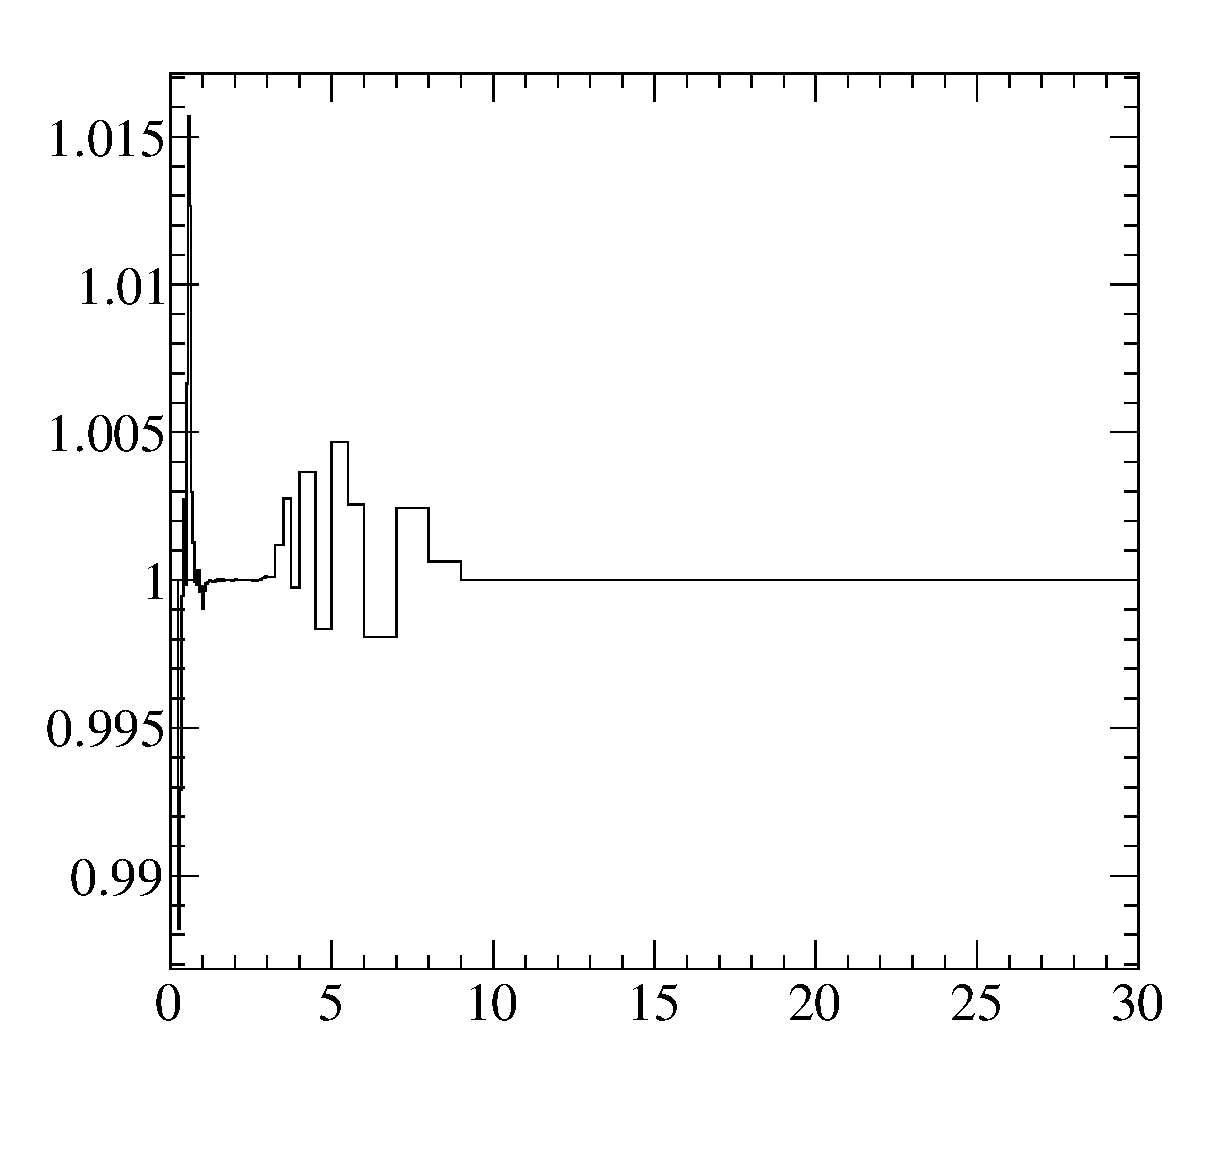
\includegraphics[width=18pc]{./images/binning/oscillation/plot_erec_int_numb_ccqe_fine}
\caption
 {Ratio of SuperK MC $E_{reco}$ spectra, for mode $\bar{\nu_\mu}$ CCQE made with 84 bin $E_{true}$ and 780 bin $E_{true}$, for an exposure of 3.010$	imes$10$^{20}$ POT. The number of events was calculated using the BANFF-tuned MC templates.Using oscillation parameters:  $\sin^22\theta_{12} = $0.857; $\sin^22\theta_{13} = $0.098; $\sin^22\theta_{23} = $1; $\delta_{CP} = $        0; $\Delta m^2_{21} = $    7.5e-05 $eV^2/c^4$; $|\Delta m^2_{32}| = $    0.0024 $eV^2/c^4$. }
\label{fig:etruebin:numubarccqe}
\end{minipage}
\hspace{0.06\linewidth}
\begin{minipage}[t]{0.48\linewidth}
\center
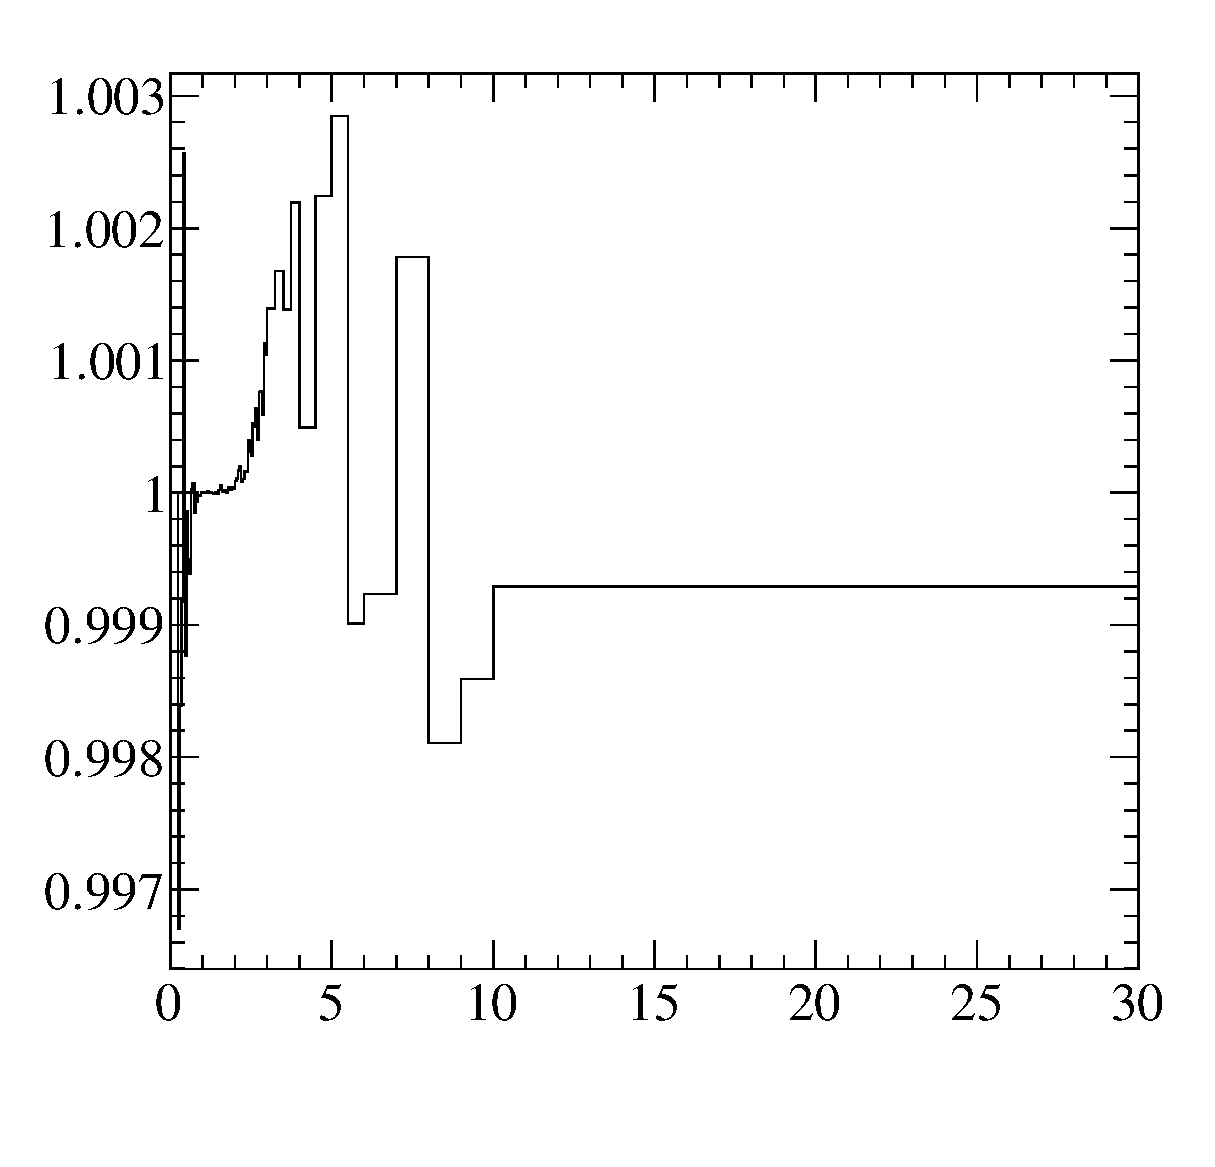
\includegraphics[width=18pc]{./images/binning/oscillation/plot_erec_int_numb_ccpi_fine}
\caption
 {Ratio of SuperK MC $E_{reco}$ spectra, for mode $\bar{\nu_\mu}$ CC 1$\pi$ made with 84 bin $E_{true}$ and 780 bin $E_{true}$, for an exposure of 3.010$	imes$10$^{20}$ POT. The number of events was calculated using the BANFF-tuned MC templates.Using oscillation parameters:  $\sin^22\theta_{12} = $0.857; $\sin^22\theta_{13} = $0.098; $\sin^22\theta_{23} = $1; $\delta_{CP} = $        0; $\Delta m^2_{21} = $    7.5e-05 $eV^2/c^4$; $|\Delta m^2_{32}| = $    0.0024 $eV^2/c^4$. }
\label{fig:etruebin:numubarcc1pi}
\end{minipage}
\vfill
\begin{minipage}[t]{0.48\linewidth}
\center
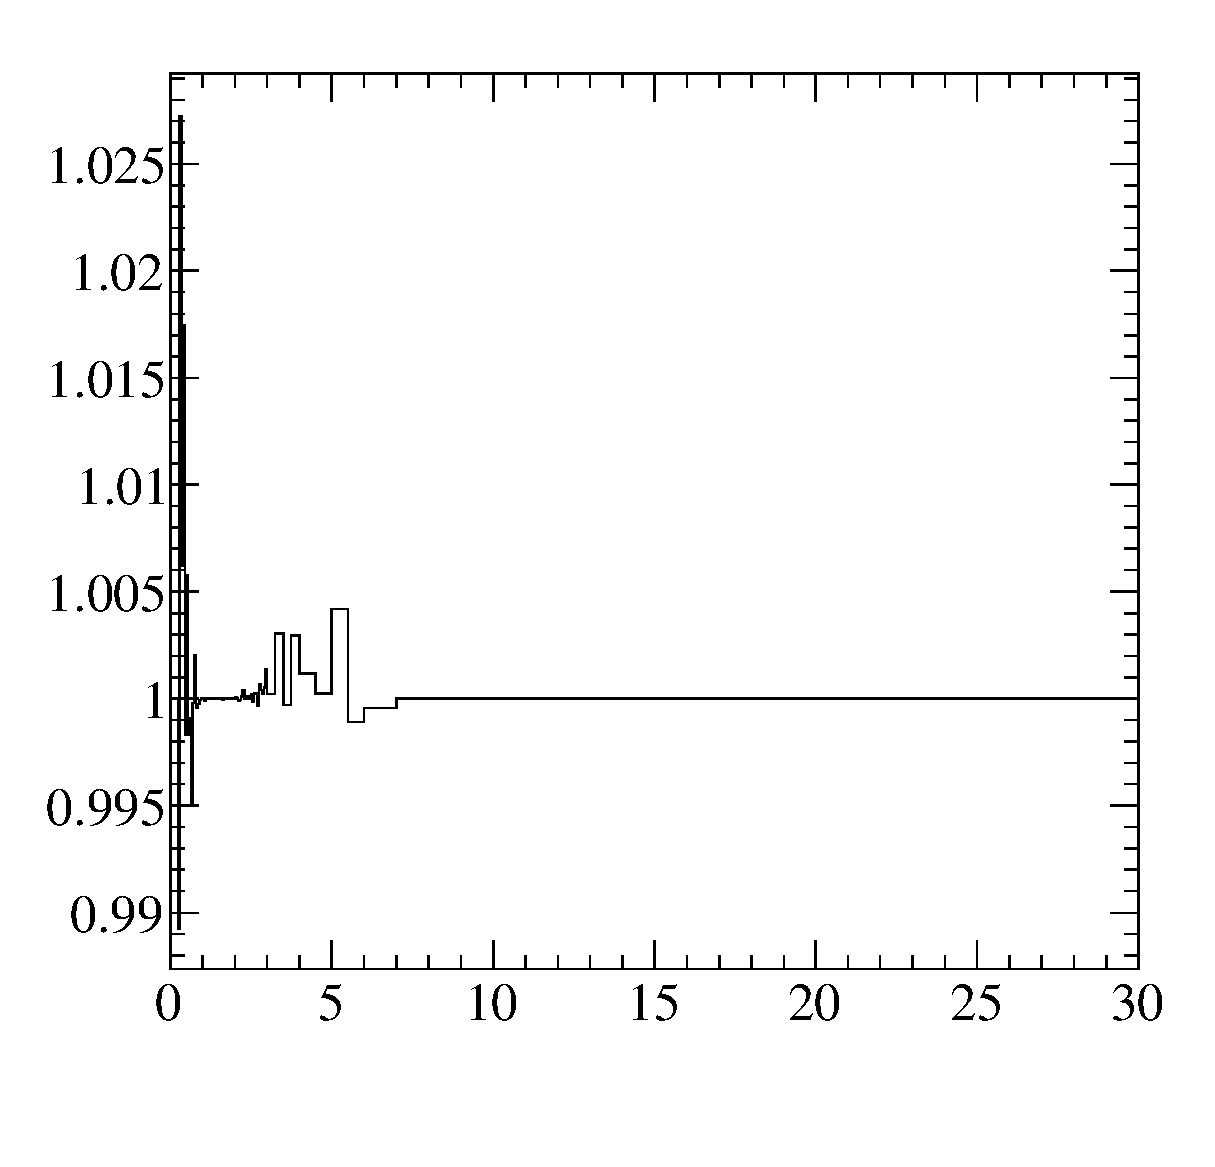
\includegraphics[width=18pc]{./images/binning/oscillation/plot_erec_int_numb_cccoh_fine}
\caption
 {Ratio of SuperK MC $E_{reco}$ spectra, for mode $\bar{\nu_\mu}$ CC coherent made with 84 bin $E_{true}$ and 780 bin $E_{true}$, for an exposure of 3.010$	imes$10$^{20}$ POT. The number of events was calculated using the BANFF-tuned MC templates.Using oscillation parameters:  $\sin^22\theta_{12} = $0.857; $\sin^22\theta_{13} = $0.098; $\sin^22\theta_{23} = $1; $\delta_{CP} = $        0; $\Delta m^2_{21} = $    7.5e-05 $eV^2/c^4$; $|\Delta m^2_{32}| = $    0.0024 $eV^2/c^4$. }
\label{fig:etruebin:numubarcccoh}
\end{minipage}
\hspace{0.06\linewidth}
\begin{minipage}[t]{0.48\linewidth}
\center
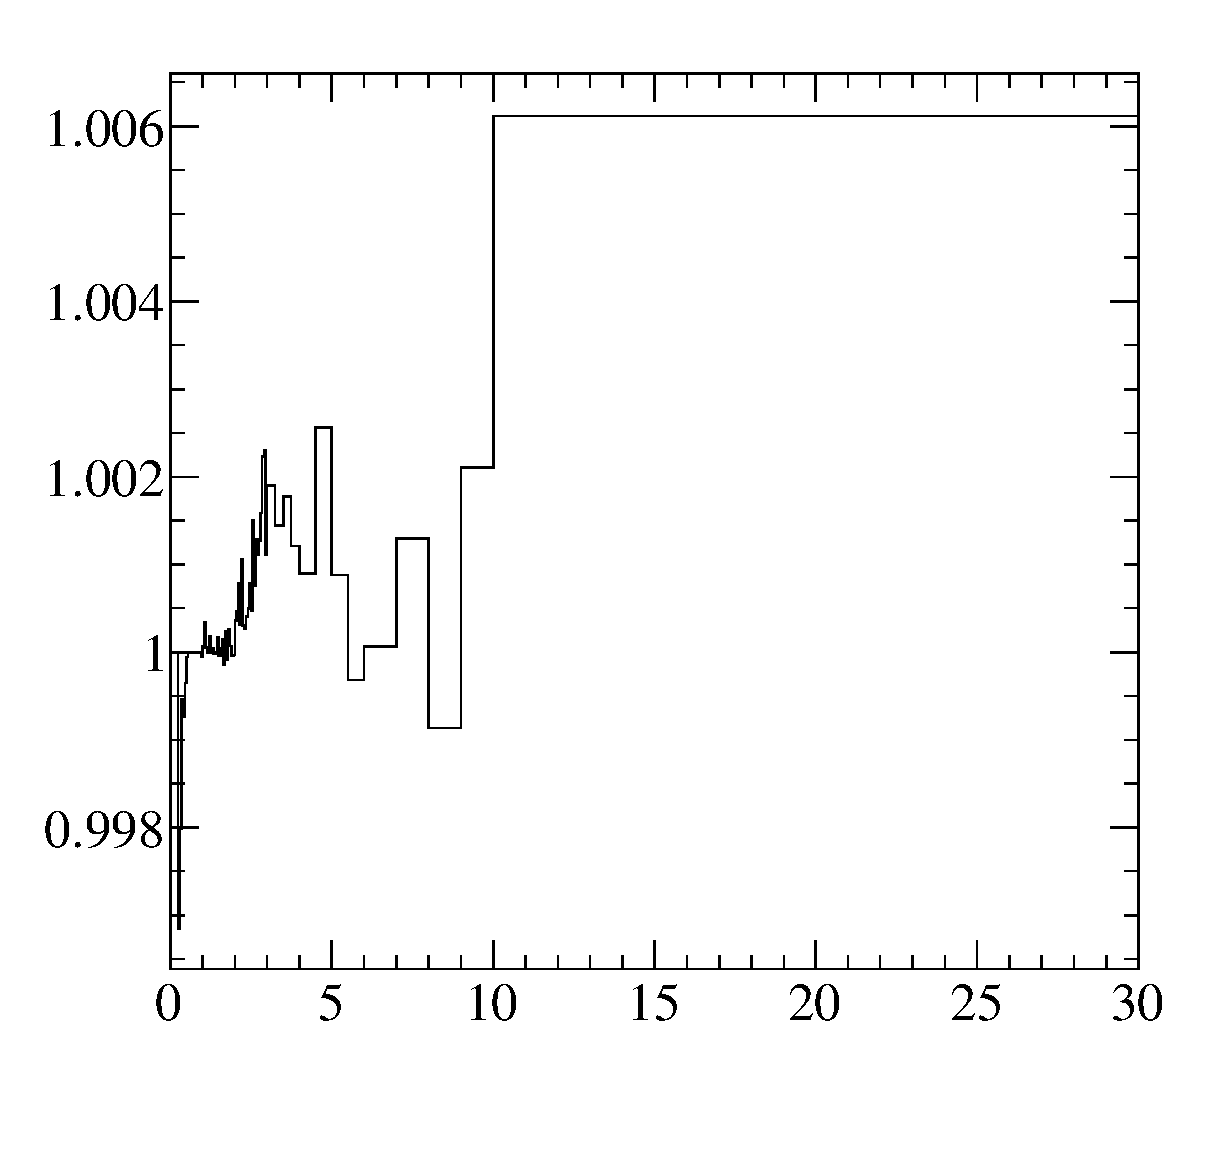
\includegraphics[width=18pc]{./images/binning/oscillation/plot_erec_int_numb_ccoth_fine}
\caption
 {Ratio of SuperK MC $E_{reco}$ spectra, for mode $\bar{\nu_\mu}$ CC other ($\nu_\mu$ disap) made with 84 bin $E_{true}$ and 780 bin $E_{true}$, for an exposure of 3.010$	imes$10$^{20}$ POT. The number of events was calculated using the BANFF-tuned MC templates.Using oscillation parameters:  $\sin^22\theta_{12} = $0.857; $\sin^22\theta_{13} = $0.098; $\sin^22\theta_{23} = $1; $\delta_{CP} = $        0; $\Delta m^2_{21} = $    7.5e-05 $eV^2/c^4$; $|\Delta m^2_{32}| = $    0.0024 $eV^2/c^4$. }
\label{fig:etruebin:numubarccoth}
\end{minipage}
\end{figure*}

%\clearpage
\begin{figure*}[htb]
\begin{minipage}[t]{0.48\linewidth}
\center
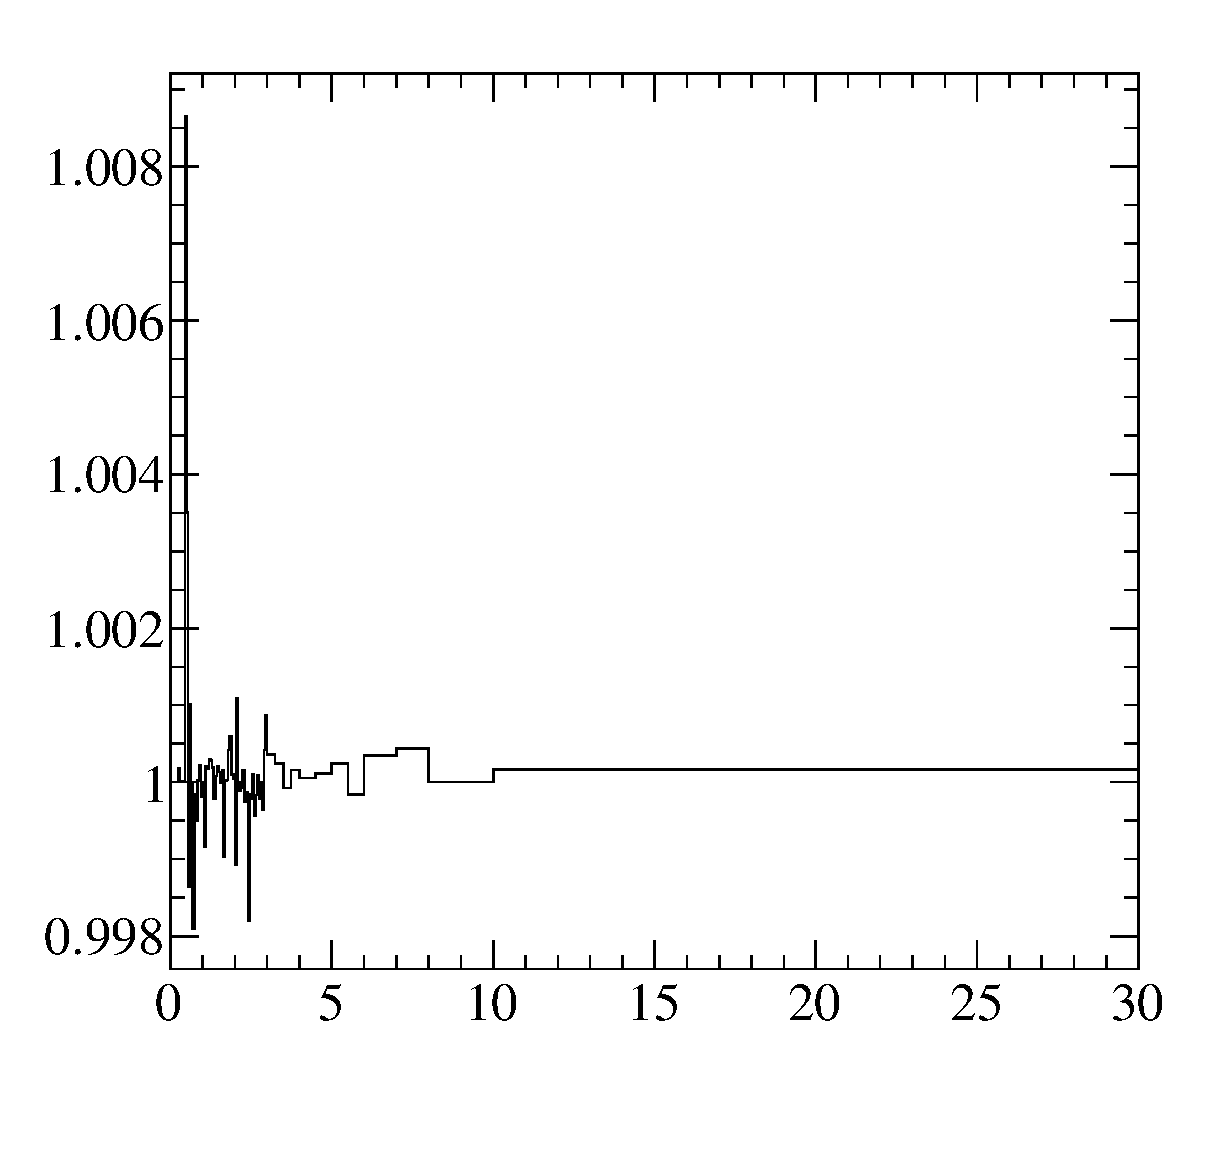
\includegraphics[width=18pc]{./images/binning/oscillation/plot_erec_int_nue_ccqe_fine}
\caption
 {Ratio of SuperK MC $E_{reco}$ spectra, for mode $\nu_e$ CCQE made with 84 bin $E_{true}$ and 780 bin $E_{true}$, for an exposure of 3.010$	imes$10$^{20}$ POT. The number of events was calculated using the BANFF-tuned MC templates.Using oscillation parameters:  $\sin^22\theta_{12} = $0.857; $\sin^22\theta_{13} = $0.098; $\sin^22\theta_{23} = $1; $\delta_{CP} = $        0; $\Delta m^2_{21} = $    7.5e-05 $eV^2/c^4$; $|\Delta m^2_{32}| = $    0.0024 $eV^2/c^4$. }
\label{fig:etruebin:nueccqe}
\end{minipage}
\hspace{0.06\linewidth}
\begin{minipage}[t]{0.48\linewidth}
\center
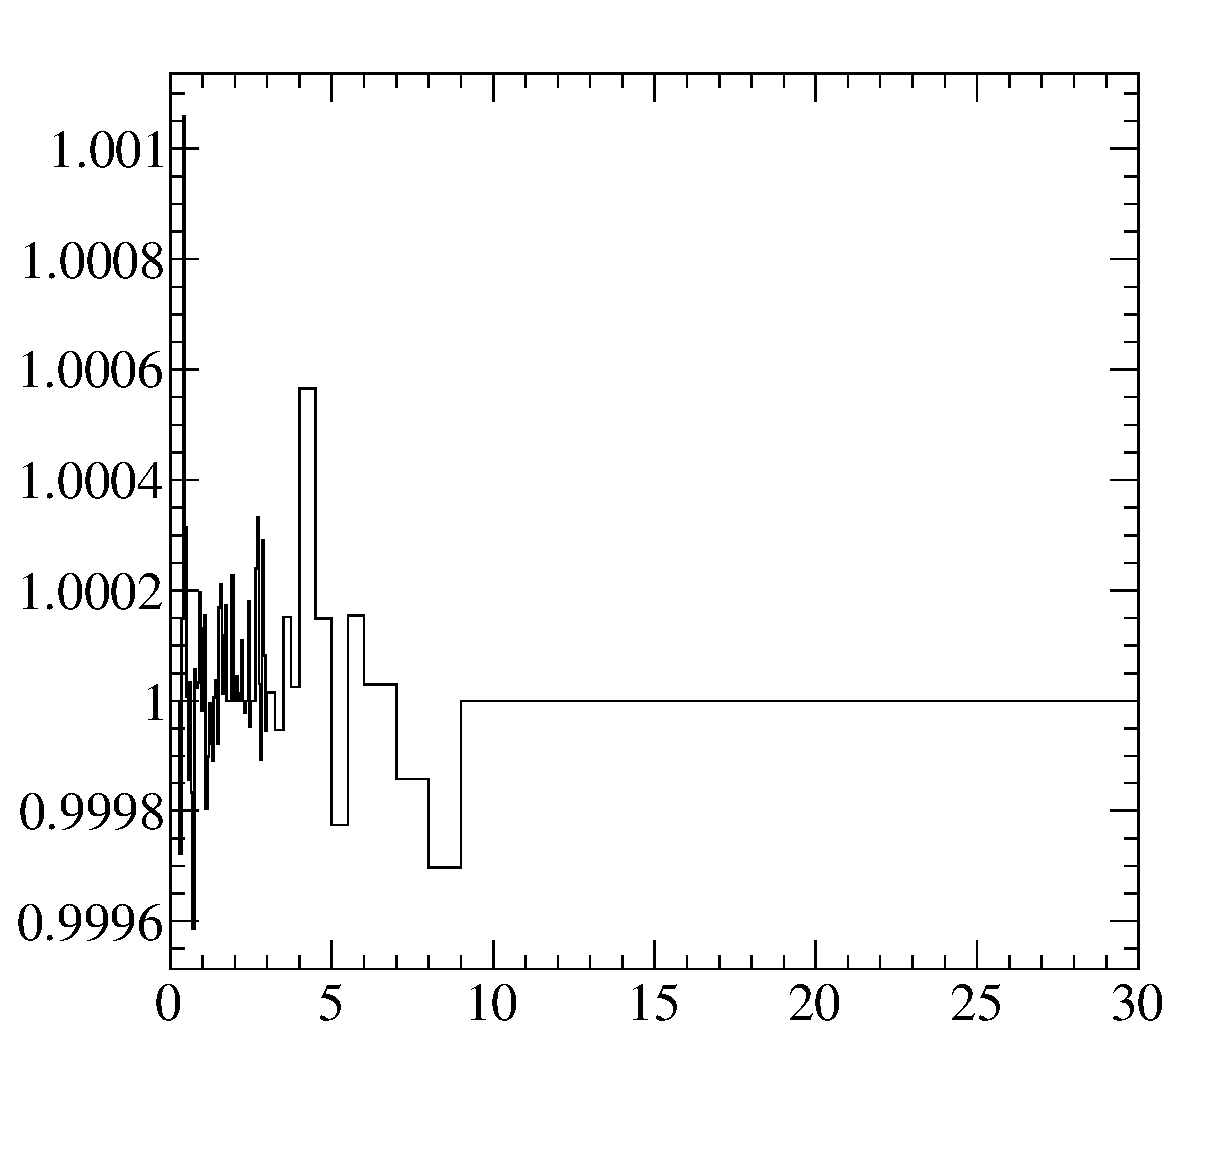
\includegraphics[width=18pc]{./images/binning/oscillation/plot_erec_int_nue_ccpi_fine}
\caption
 {Ratio of SuperK MC $E_{reco}$ spectra, for mode $\nu_e$ CC 1$\pi$ made with 84 bin $E_{true}$ and 780 bin $E_{true}$, for an exposure of 3.010$	imes$10$^{20}$ POT. The number of events was calculated using the BANFF-tuned MC templates.Using oscillation parameters:  $\sin^22\theta_{12} = $0.857; $\sin^22\theta_{13} = $0.098; $\sin^22\theta_{23} = $1; $\delta_{CP} = $        0; $\Delta m^2_{21} = $    7.5e-05 $eV^2/c^4$; $|\Delta m^2_{32}| = $    0.0024 $eV^2/c^4$. }
\label{fig:etruebin:nuecc1pi}
\end{minipage}
\vfill
\begin{minipage}[t]{0.48\linewidth}
\center
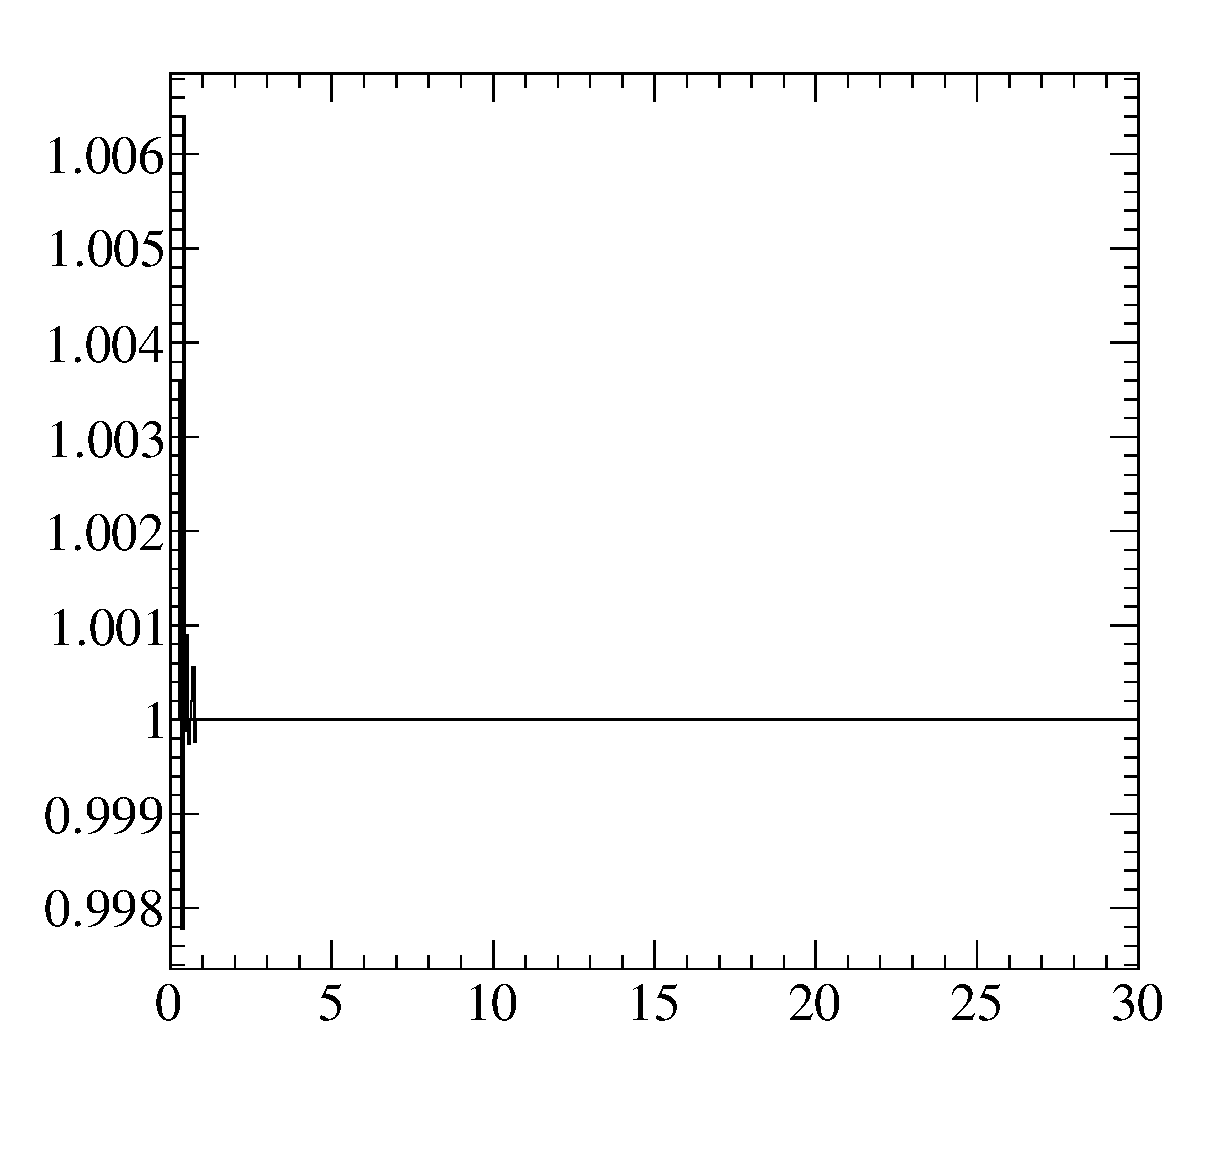
\includegraphics[width=18pc]{./images/binning/oscillation/plot_erec_int_nue_cccoh_fine}
\caption
 {Ratio of SuperK MC $E_{reco}$ spectra, for mode $\nu_e$ CC coherent made with 84 bin $E_{true}$ and 780 bin $E_{true}$, for an exposure of 3.010$	imes$10$^{20}$ POT. The number of events was calculated using the BANFF-tuned MC templates.Using oscillation parameters:  $\sin^22\theta_{12} = $0.857; $\sin^22\theta_{13} = $0.098; $\sin^22\theta_{23} = $1; $\delta_{CP} = $        0; $\Delta m^2_{21} = $    7.5e-05 $eV^2/c^4$; $|\Delta m^2_{32}| = $    0.0024 $eV^2/c^4$. }
\label{fig:etruebin:nuecccoh}
\end{minipage}
\hspace{0.06\linewidth}
\begin{minipage}[t]{0.48\linewidth}
\center
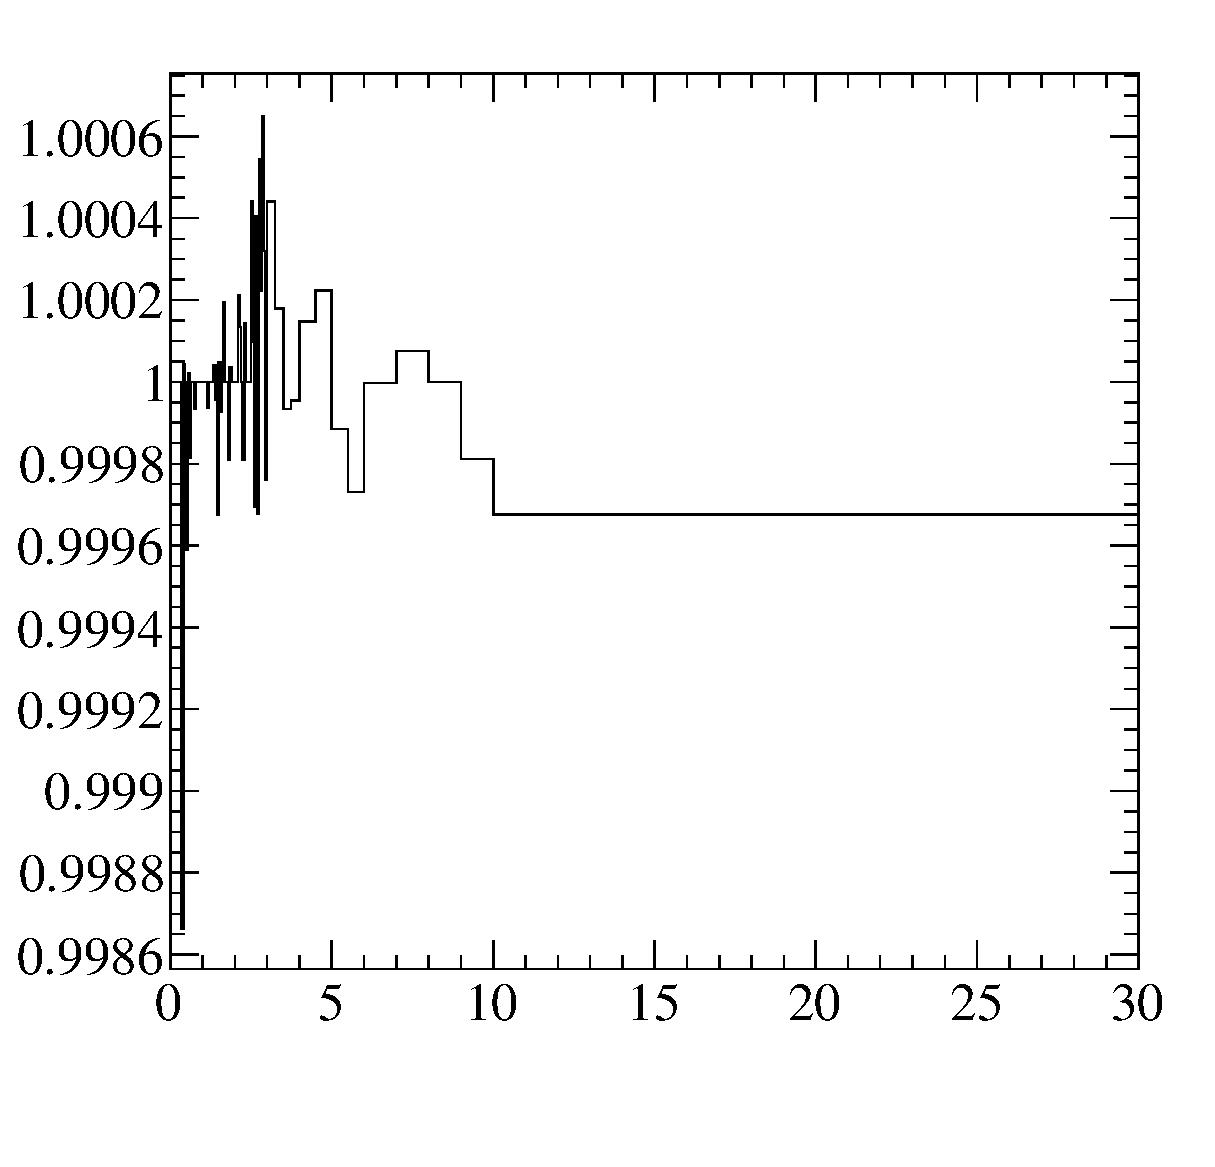
\includegraphics[width=18pc]{./images/binning/oscillation/plot_erec_int_nue_ccoth_fine}
\caption
 {Ratio of SuperK MC $E_{reco}$ spectra, for mode $\nu_e$ CC other ($\nu_\mu$ disap) made with 84 bin $E_{true}$ and 780 bin $E_{true}$, for an exposure of 3.010$	imes$10$^{20}$ POT. The number of events was calculated using the BANFF-tuned MC templates.Using oscillation parameters:  $\sin^22\theta_{12} = $0.857; $\sin^22\theta_{13} = $0.098; $\sin^22\theta_{23} = $1; $\delta_{CP} = $        0; $\Delta m^2_{21} = $    7.5e-05 $eV^2/c^4$; $|\Delta m^2_{32}| = $    0.0024 $eV^2/c^4$. }
\label{fig:etruebin:nueccoth}
\end{minipage}
\end{figure*}

%\clearpage
\begin{figure*}[htb]
\begin{minipage}[t]{0.48\linewidth}
\center
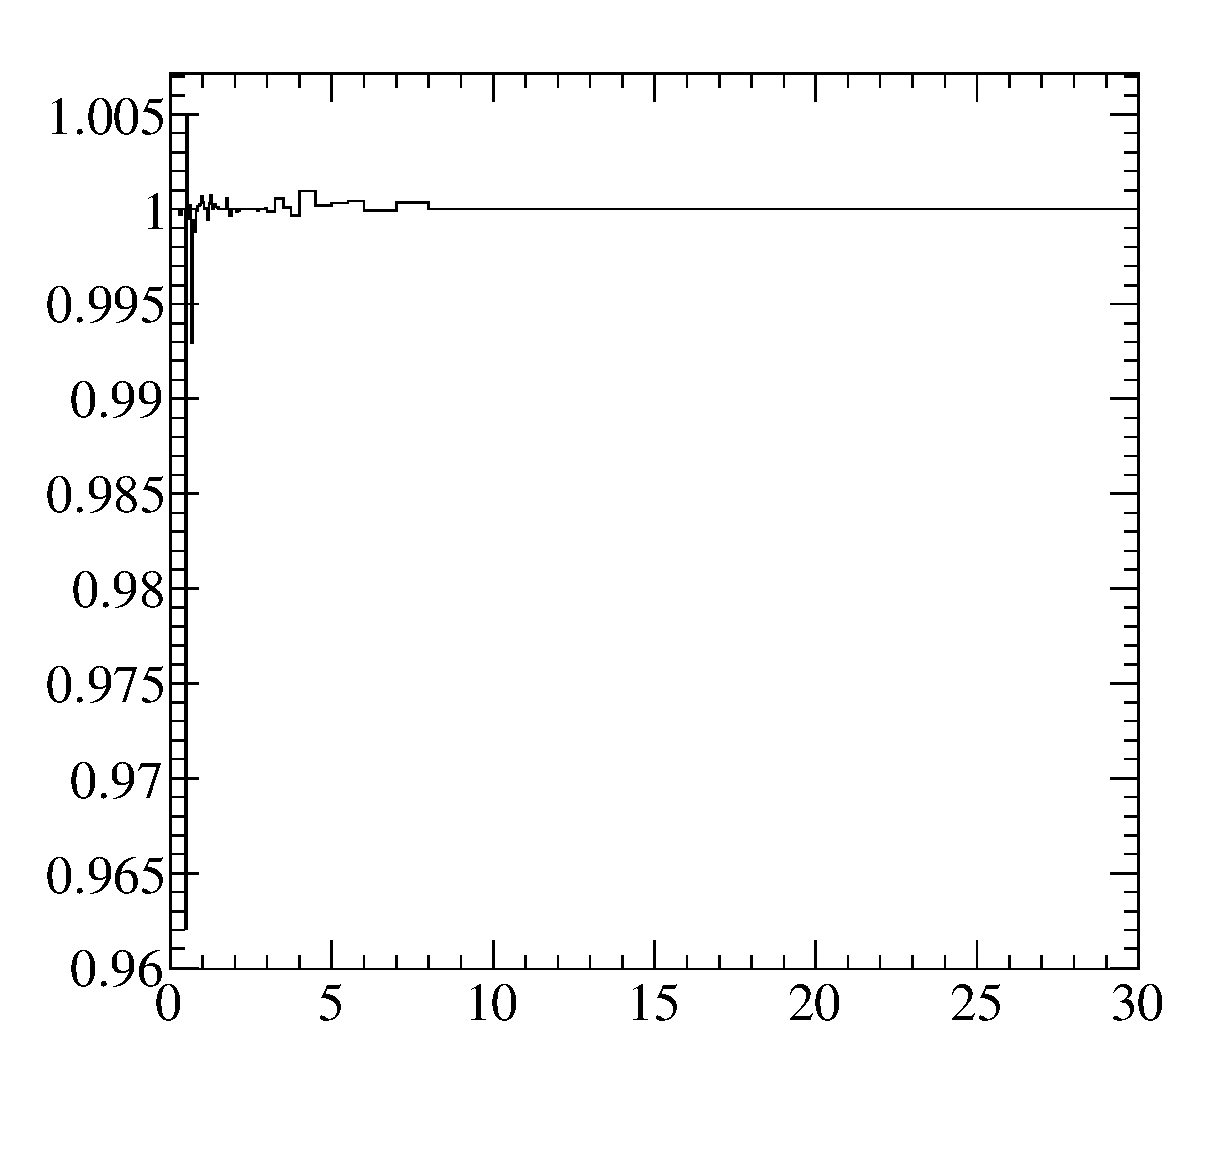
\includegraphics[width=18pc]{./images/binning/oscillation/plot_erec_int_nueb_ccqe_fine}
\caption
 {Ratio of SuperK MC $E_{reco}$ spectra, for mode $\bar{\nu_e}$ CCQE made with 84 bin $E_{true}$ and 780 bin $E_{true}$, for an exposure of 3.010$	imes$10$^{20}$ POT. The number of events was calculated using the BANFF-tuned MC templates.Using oscillation parameters:  $\sin^22\theta_{12} = $0.857; $\sin^22\theta_{13} = $0.098; $\sin^22\theta_{23} = $1; $\delta_{CP} = $        0; $\Delta m^2_{21} = $    7.5e-05 $eV^2/c^4$; $|\Delta m^2_{32}| = $    0.0024 $eV^2/c^4$. }
\label{fig:etruebin:nuebarccqe}
\end{minipage}
\hspace{0.06\linewidth}
\begin{minipage}[t]{0.48\linewidth}
\center
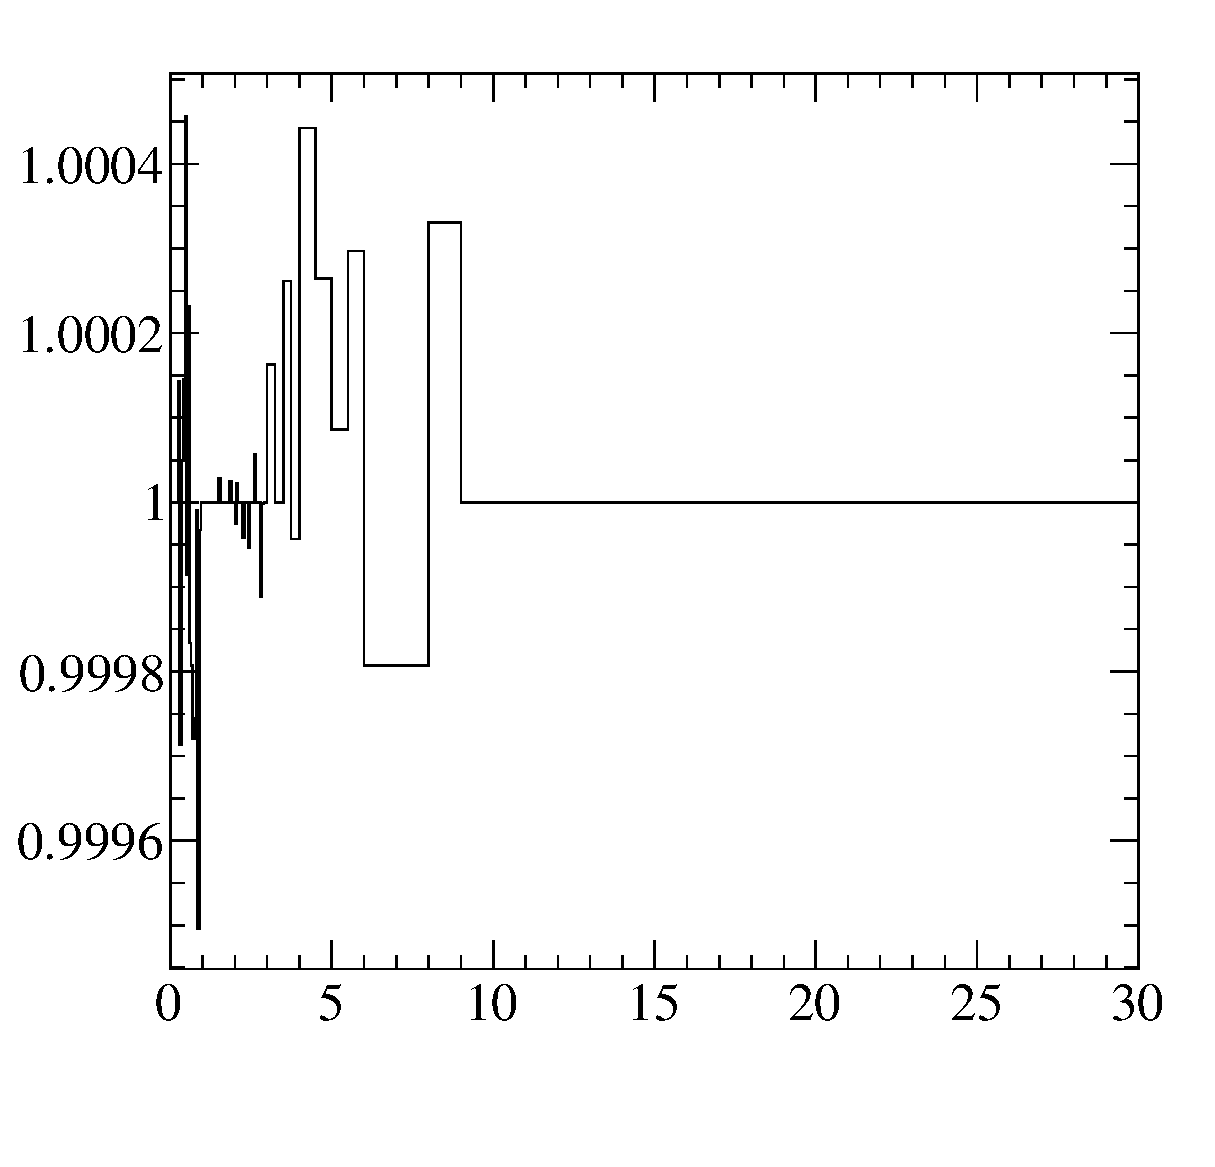
\includegraphics[width=18pc]{./images/binning/oscillation/plot_erec_int_nueb_ccpi_fine}
\caption
 {Ratio of SuperK MC $E_{reco}$ spectra, for mode $\bar{\nu_e}$ CC 1$\pi$ made with 84 bin $E_{true}$ and 780 bin $E_{true}$, for an exposure of 3.010$	imes$10$^{20}$ POT. The number of events was calculated using the BANFF-tuned MC templates.Using oscillation parameters:  $\sin^22\theta_{12} = $0.857; $\sin^22\theta_{13} = $0.098; $\sin^22\theta_{23} = $1; $\delta_{CP} = $        0; $\Delta m^2_{21} = $    7.5e-05 $eV^2/c^4$; $|\Delta m^2_{32}| = $    0.0024 $eV^2/c^4$. }
\label{fig:etruebin:nuebarcc1pi}
\end{minipage}
\vfill
\begin{minipage}[t]{0.48\linewidth}
\center
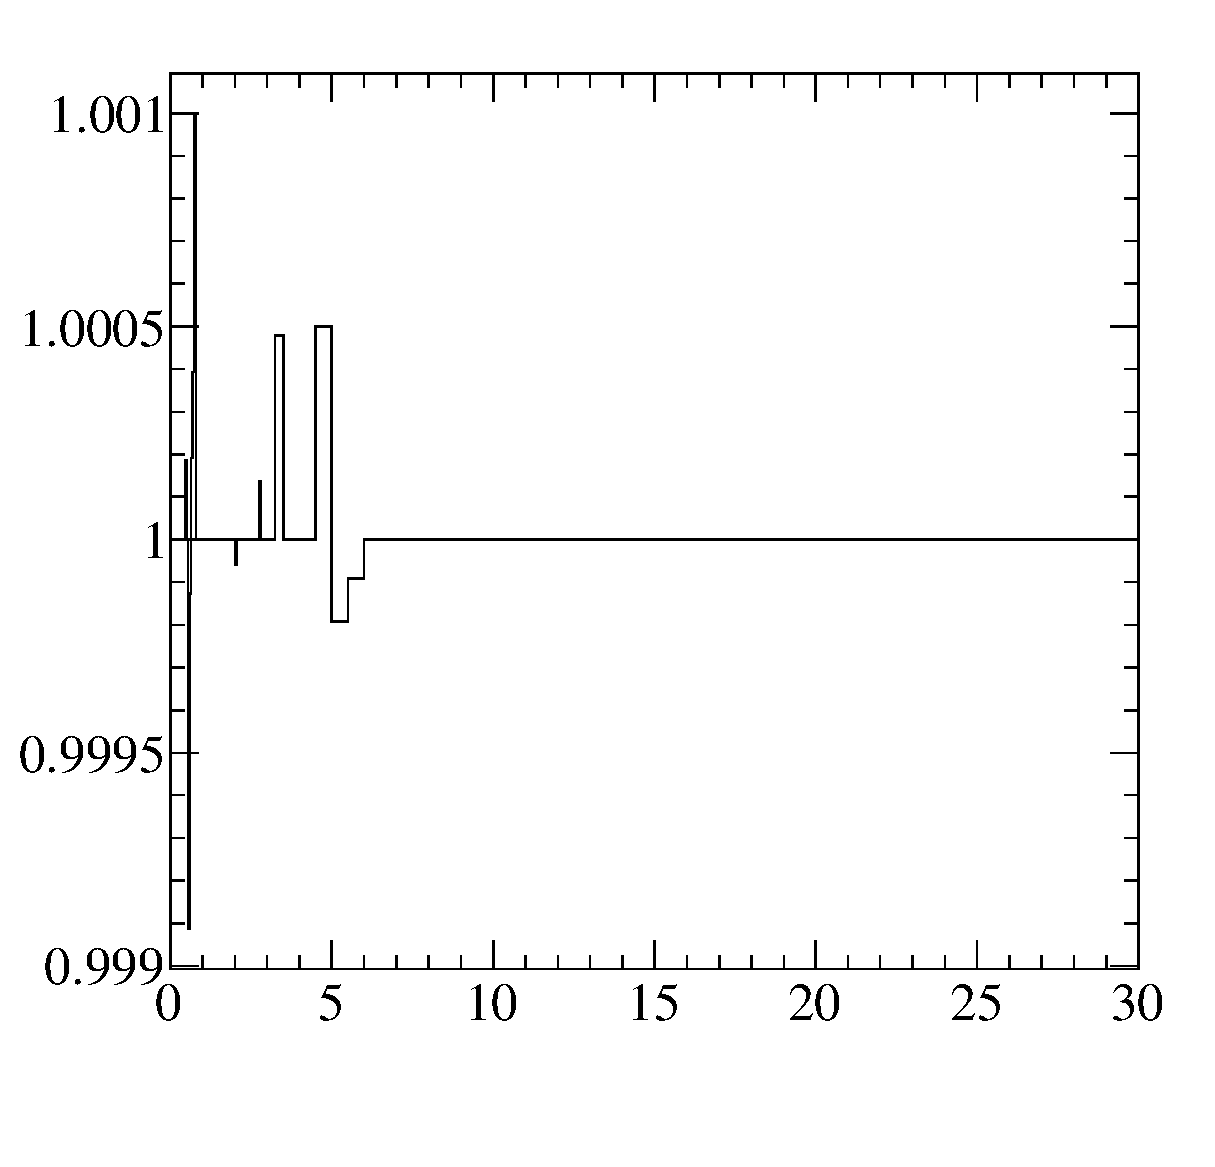
\includegraphics[width=18pc]{./images/binning/oscillation/plot_erec_int_nueb_cccoh_fine}
\caption
 {Ratio of SuperK MC $E_{reco}$ spectra, for mode $\bar{\nu_e}$ CC coherent made with 84 bin $E_{true}$ and 780 bin $E_{true}$, for an exposure of 3.010$	imes$10$^{20}$ POT. The number of events was calculated using the BANFF-tuned MC templates.Using oscillation parameters:  $\sin^22\theta_{12} = $0.857; $\sin^22\theta_{13} = $0.098; $\sin^22\theta_{23} = $1; $\delta_{CP} = $        0; $\Delta m^2_{21} = $    7.5e-05 $eV^2/c^4$; $|\Delta m^2_{32}| = $    0.0024 $eV^2/c^4$. }
\label{fig:etruebin:nuebarcccoh}
\end{minipage}
\hspace{0.06\linewidth}
\begin{minipage}[t]{0.48\linewidth}
\center
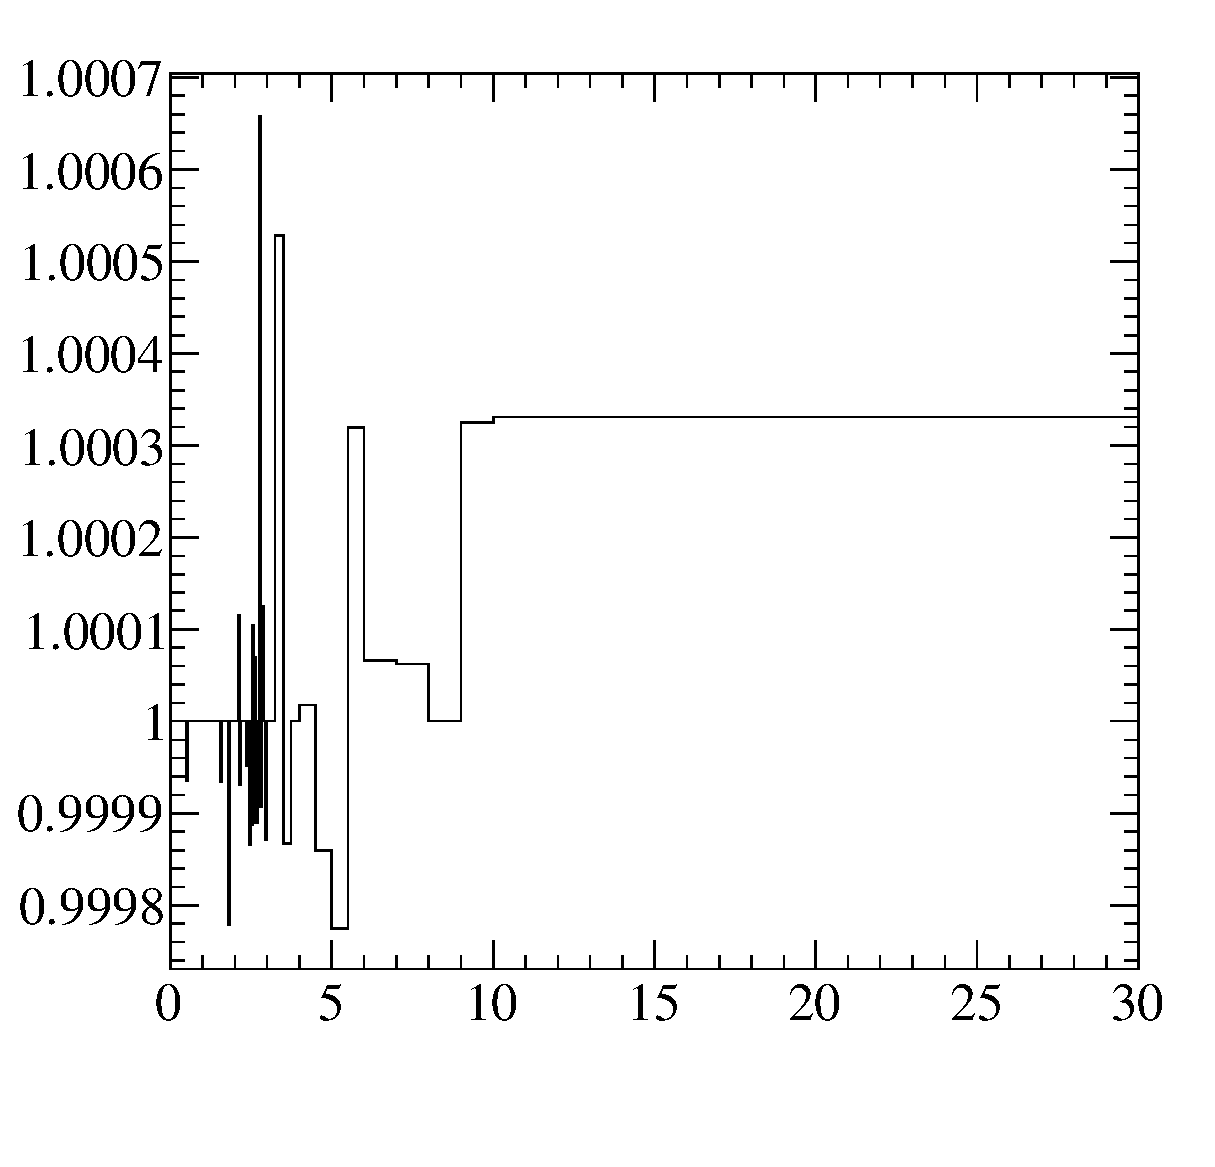
\includegraphics[width=18pc]{./images/binning/oscillation/plot_erec_int_nueb_ccoth_fine}
\caption
 {Ratio of SuperK MC $E_{reco}$ spectra, for mode $\bar{\nu_e}$ CC other ($\nu_\mu$ disap) made with 84 bin $E_{true}$ and 780 bin $E_{true}$, for an exposure of 3.010$	imes$10$^{20}$ POT. The number of events was calculated using the BANFF-tuned MC templates.Using oscillation parameters:  $\sin^22\theta_{12} = $0.857; $\sin^22\theta_{13} = $0.098; $\sin^22\theta_{23} = $1; $\delta_{CP} = $        0; $\Delta m^2_{21} = $    7.5e-05 $eV^2/c^4$; $|\Delta m^2_{32}| = $    0.0024 $eV^2/c^4$. }
\label{fig:etruebin:nuebarccoth}
\end{minipage}
\end{figure*}

%\clearpage
\begin{figure*}[htb]
\begin{minipage}[t]{0.48\linewidth}
\center
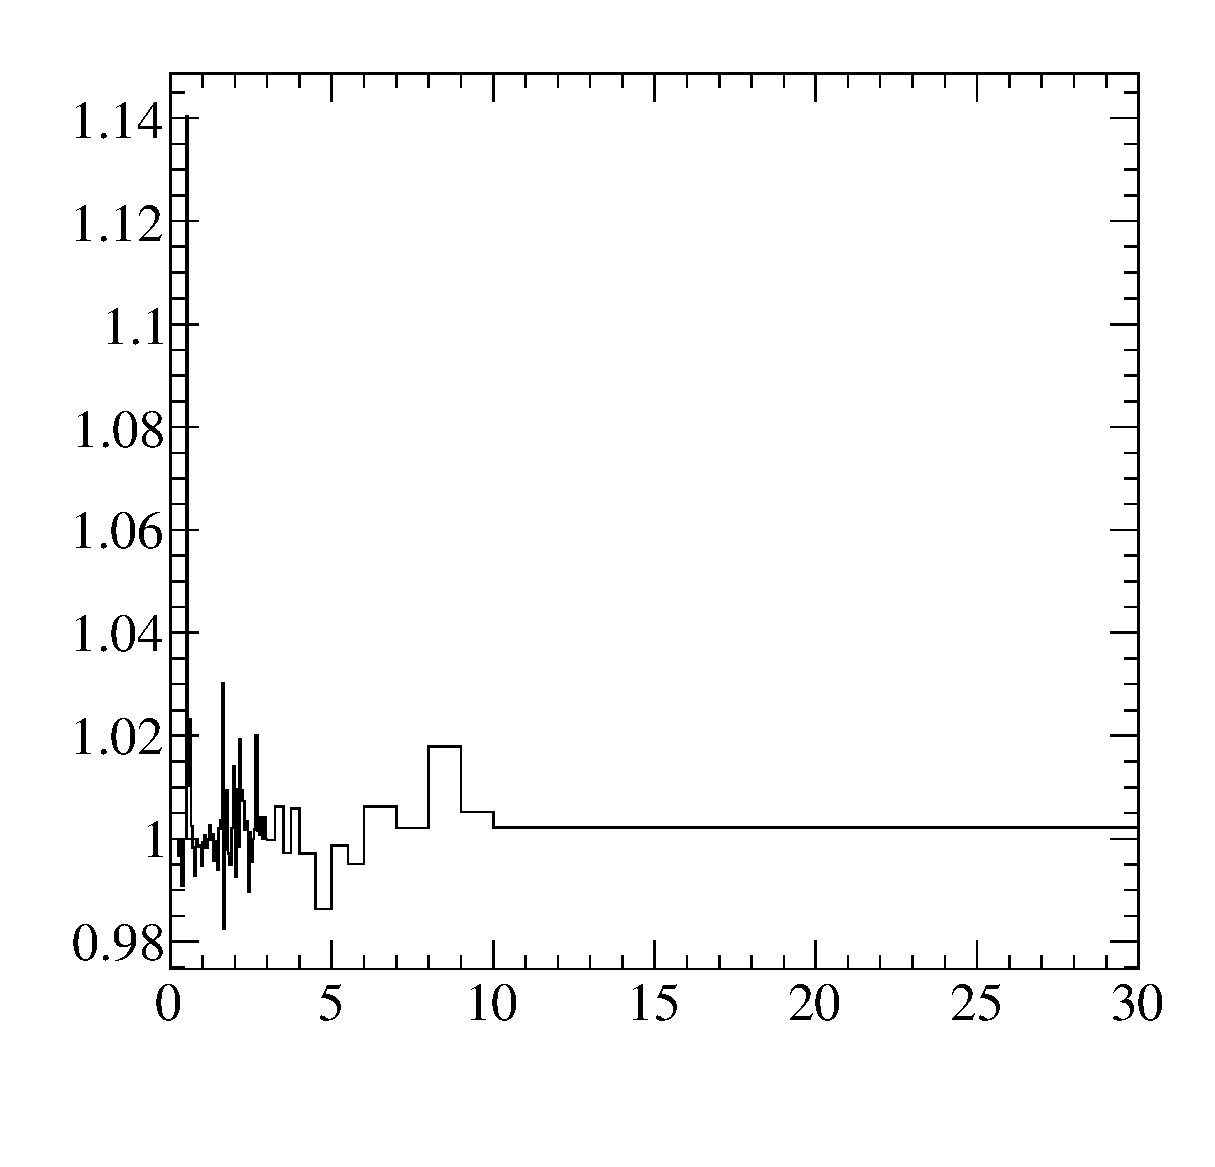
\includegraphics[width=18pc]{./images/binning/oscillation/plot_erec_int_signue_ccqe_fine}
\caption
 {Ratio of SuperK MC $E_{reco}$ spectra, for mode oscillation $\nu_e$ CCQE made with 84 bin $E_{true}$ and 780 bin $E_{true}$, for an exposure of 3.010$	imes$10$^{20}$ POT. The number of events was calculated using the BANFF-tuned MC templates.Using oscillation parameters:  $\sin^22\theta_{12} = $0.857; $\sin^22\theta_{13} = $0.098; $\sin^22\theta_{23} = $1; $\delta_{CP} = $        0; $\Delta m^2_{21} = $    7.5e-05 $eV^2/c^4$; $|\Delta m^2_{32}| = $    0.0024 $eV^2/c^4$. }
\label{fig:etruebin:signueccqe}
\end{minipage}
\hspace{0.06\linewidth}
\begin{minipage}[t]{0.48\linewidth}
\center
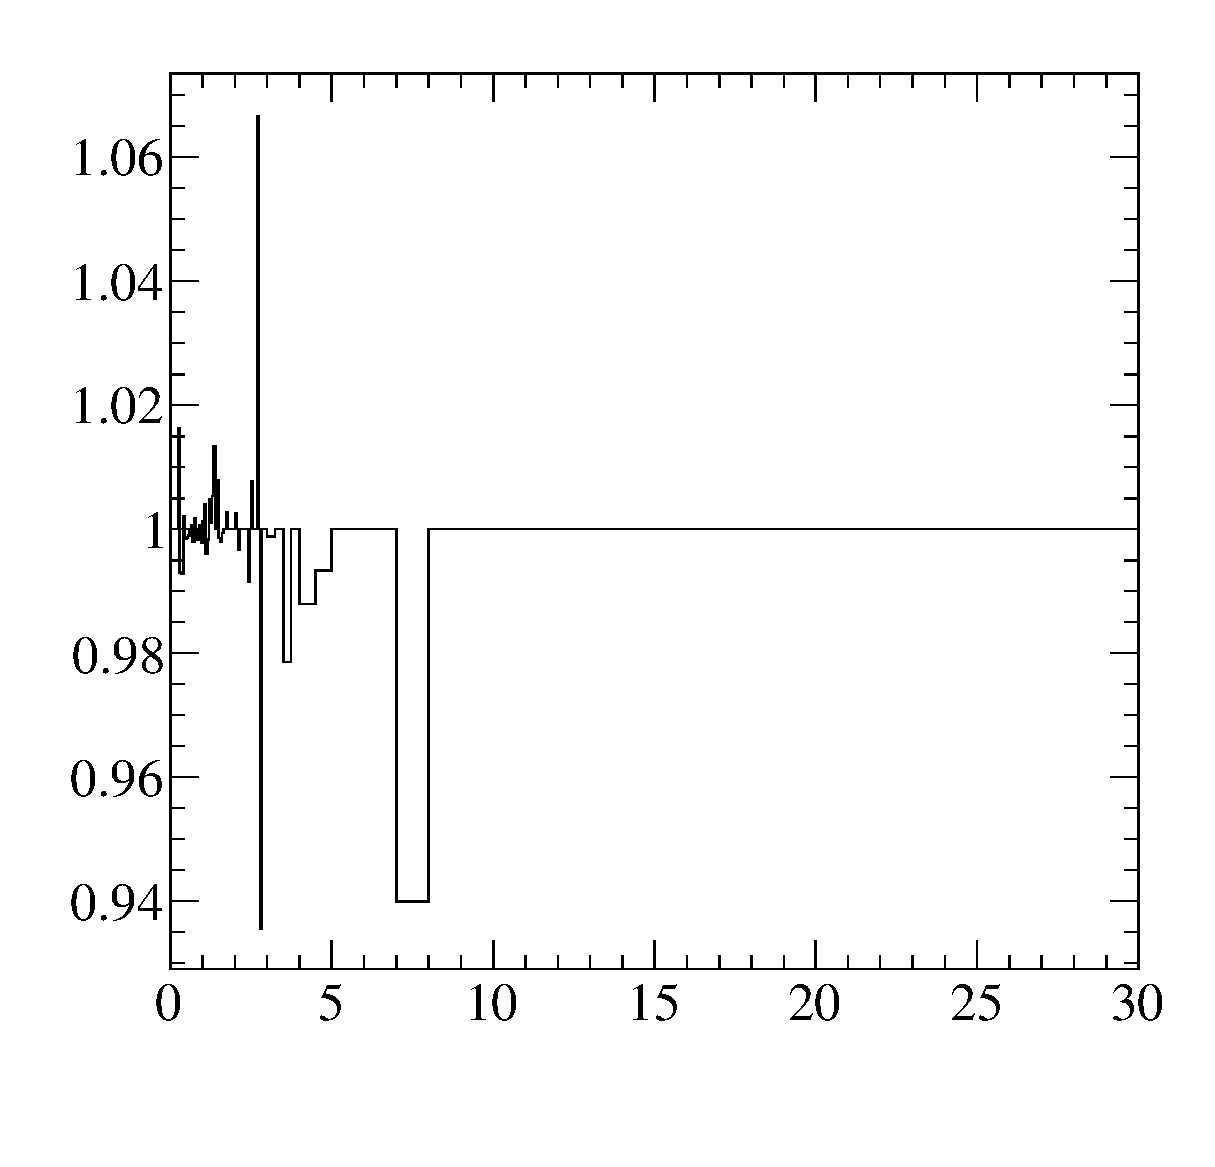
\includegraphics[width=18pc]{./images/binning/oscillation/plot_erec_int_signue_ccpi_fine}
\caption
 {Ratio of SuperK MC $E_{reco}$ spectra, for mode oscillation $\nu_e$ CC 1$\pi$ made with 84 bin $E_{true}$ and 780 bin $E_{true}$, for an exposure of 3.010$	imes$10$^{20}$ POT. The number of events was calculated using the BANFF-tuned MC templates.Using oscillation parameters:  $\sin^22\theta_{12} = $0.857; $\sin^22\theta_{13} = $0.098; $\sin^22\theta_{23} = $1; $\delta_{CP} = $        0; $\Delta m^2_{21} = $    7.5e-05 $eV^2/c^4$; $|\Delta m^2_{32}| = $    0.0024 $eV^2/c^4$. }
\label{fig:etruebin:signuecc1pi}
\end{minipage}
\vfill
\begin{minipage}[t]{0.48\linewidth}
\center
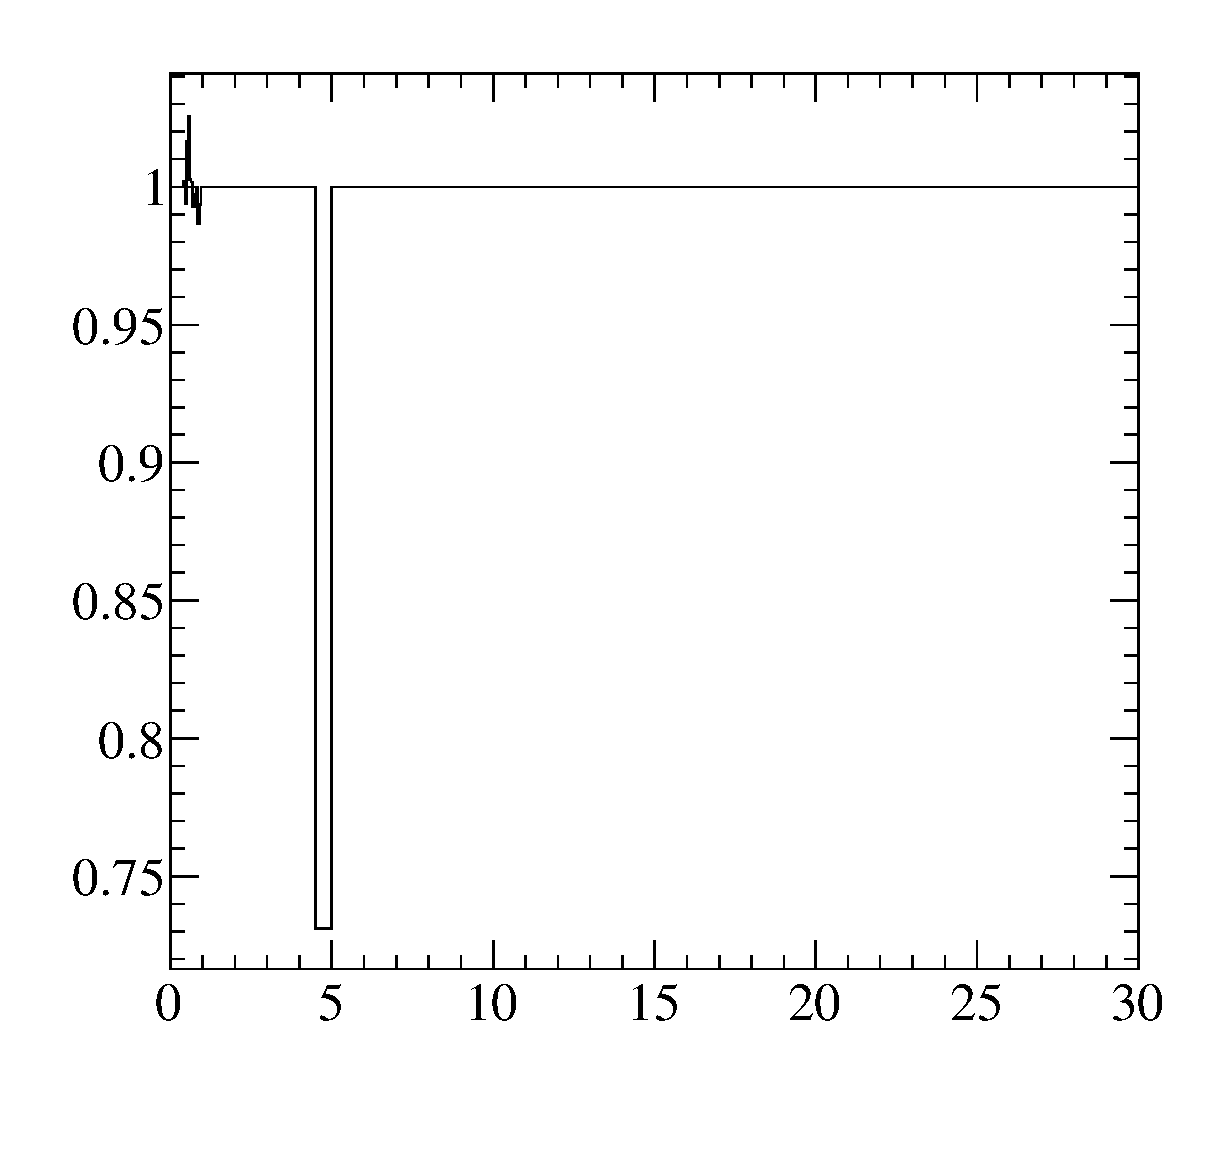
\includegraphics[width=18pc]{./images/binning/oscillation/plot_erec_int_signue_cccoh_fine}
\caption
 {Ratio of SuperK MC $E_{reco}$ spectra, for mode oscillation $\nu_e$ CC coherent made with 84 bin $E_{true}$ and 780 bin $E_{true}$, for an exposure of 3.010$	imes$10$^{20}$ POT. The number of events was calculated using the BANFF-tuned MC templates.Using oscillation parameters:  $\sin^22\theta_{12} = $0.857; $\sin^22\theta_{13} = $0.098; $\sin^22\theta_{23} = $1; $\delta_{CP} = $        0; $\Delta m^2_{21} = $    7.5e-05 $eV^2/c^4$; $|\Delta m^2_{32}| = $    0.0024 $eV^2/c^4$. }
\label{fig:etruebin:signuecccoh}
\end{minipage}
\hspace{0.06\linewidth}
\begin{minipage}[t]{0.48\linewidth}
\center
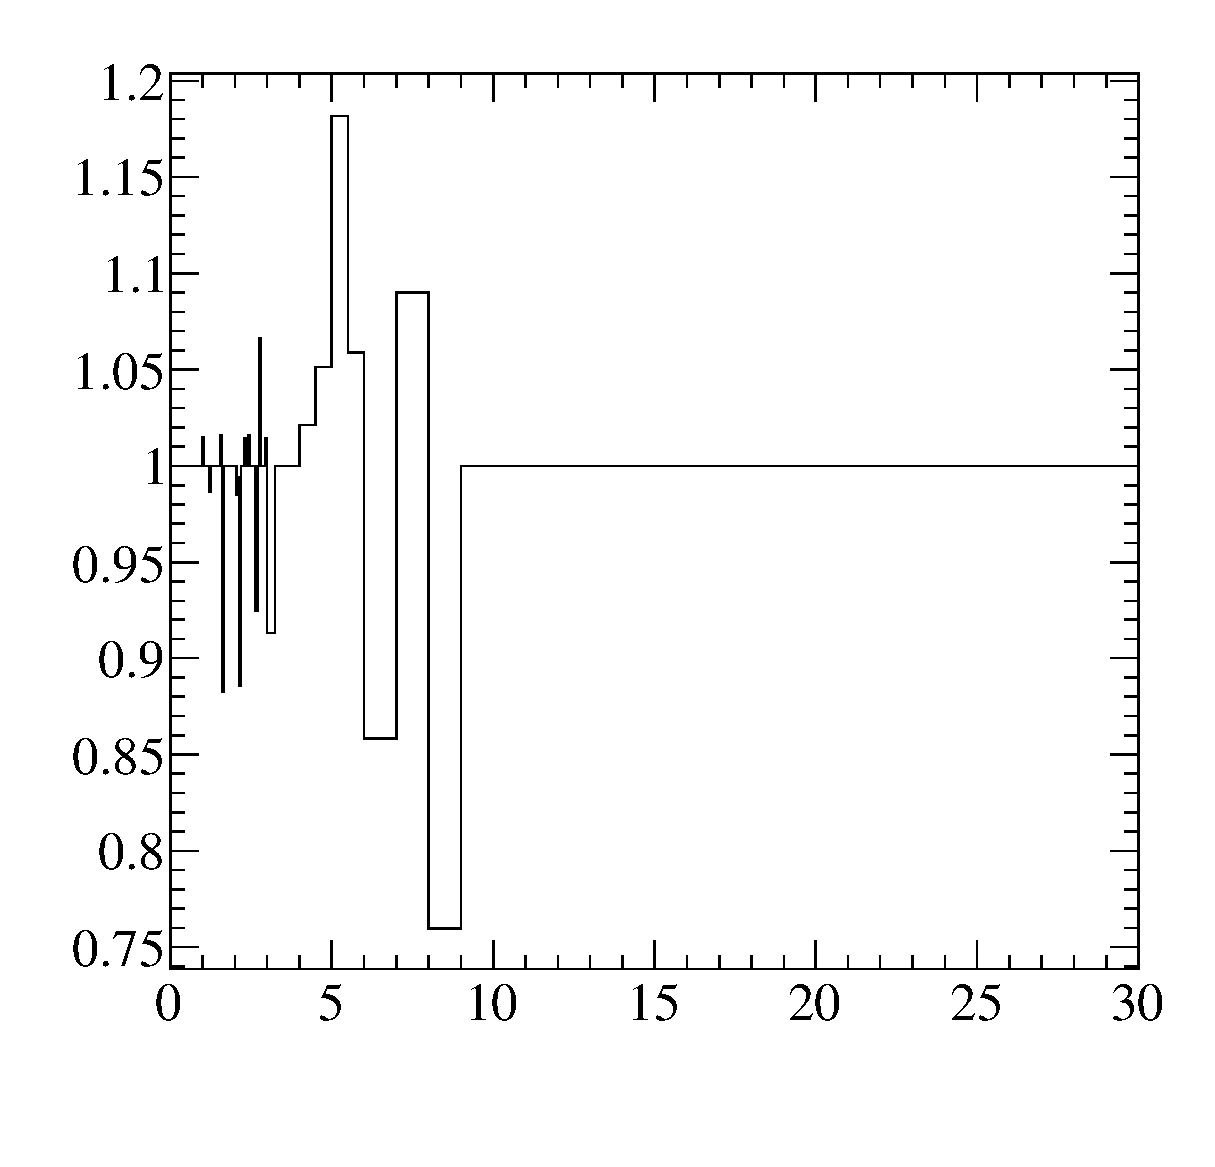
\includegraphics[width=18pc]{./images/binning/oscillation/plot_erec_int_signue_ccoth_fine}
\caption
 {Ratio of SuperK MC $E_{reco}$ spectra, for mode oscillation $\nu_e$ CC other ($\nu_\mu$ app) made with 84 bin $E_{true}$ and 780 bin $E_{true}$, for an exposure of 3.010$	imes$10$^{20}$ POT. The number of events was calculated using the BANFF-tuned MC templates.Using oscillation parameters:  $\sin^22\theta_{12} = $0.857; $\sin^22\theta_{13} = $0.098; $\sin^22\theta_{23} = $1; $\delta_{CP} = $        0; $\Delta m^2_{21} = $    7.5e-05 $eV^2/c^4$; $\Delta m^2_{32} = $    0.0024 $eV^2/c^4$. }
\label{fig:etruebin:signueccoth}
\end{minipage}
\end{figure*}

\clearpage


\begin{figure*}[htb]
\center
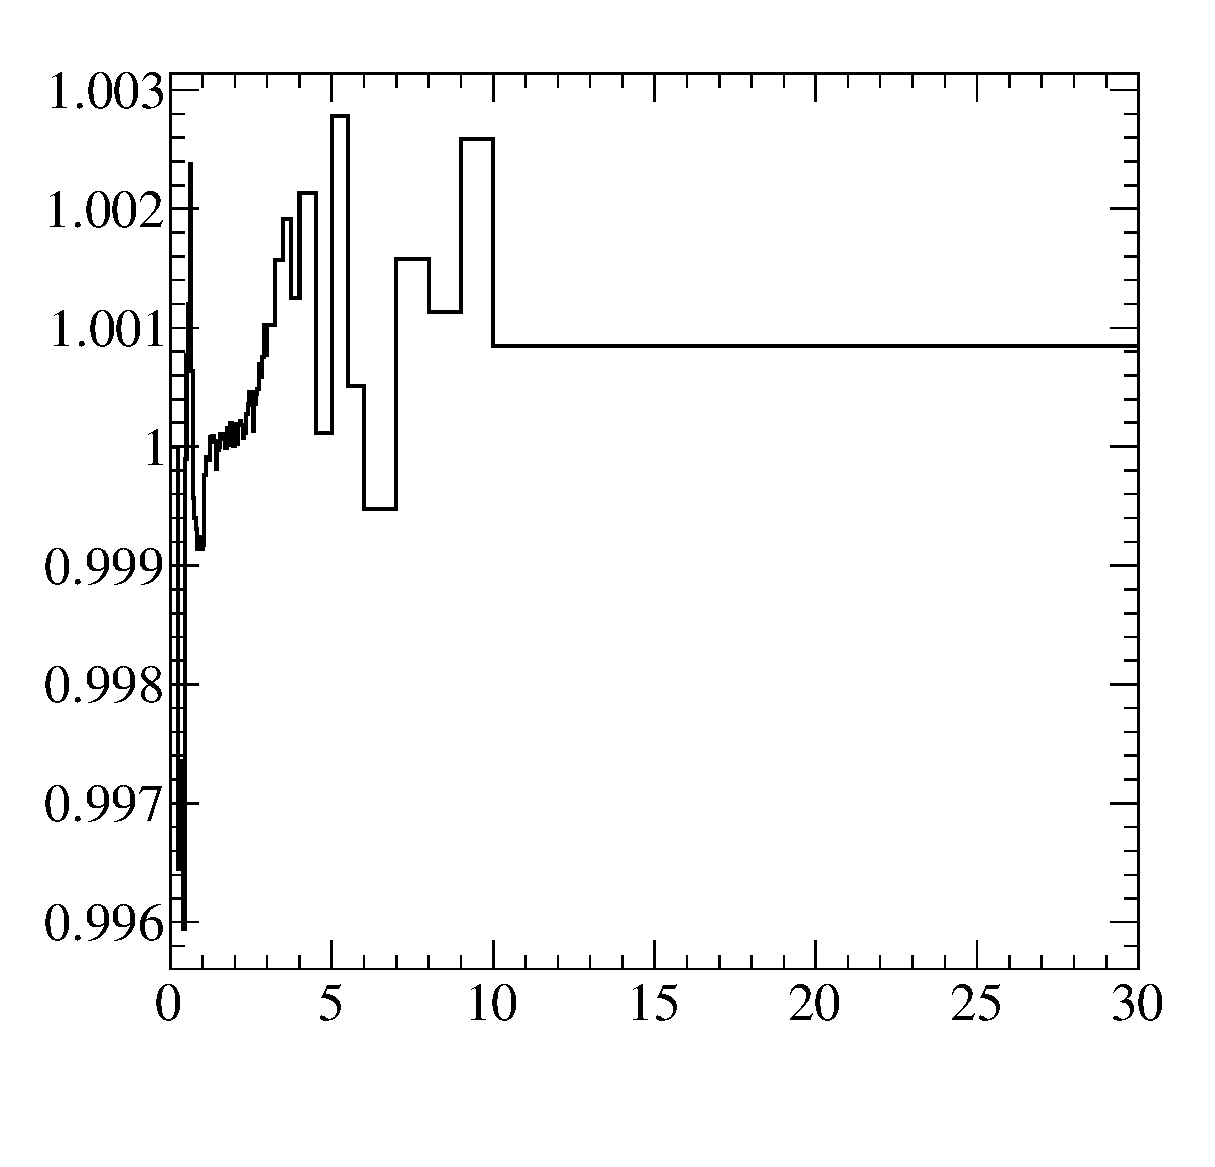
\includegraphics[width=30pc]{./images/binning/oscillation/plot_ereco_spectrum}
\caption {
  Ratio of total SuperK MC $E_{reco}$ spectra, made with 84-bin $E_{true}$ and 780-bin $E_{true}$, for an exposure of 3.010$\times$10$^{20}$ POT.
  The number of events was calculated using the BANFF-tuned MC templates.
  Using oscillation parameters:  $\sin^22\theta_{12} = $0.857; $\sin^22\theta_{13} = $0.098; $\sin^22\theta_{23} = $1; $\delta_{CP} = $        0; $\Delta m^2_{21} = $    7.5e-05 $eV^2/c^4$; $|\Delta m^2_{32}| = $    0.0024 $eV^2/c^4$.
}
\label{fig:etruebin:total}
\end{figure*}

%
% ----------------------------------------
%

%
% Figs for \subsection{$E_{reco}$ binning}
%

\begin{figure*}[htb]
\center
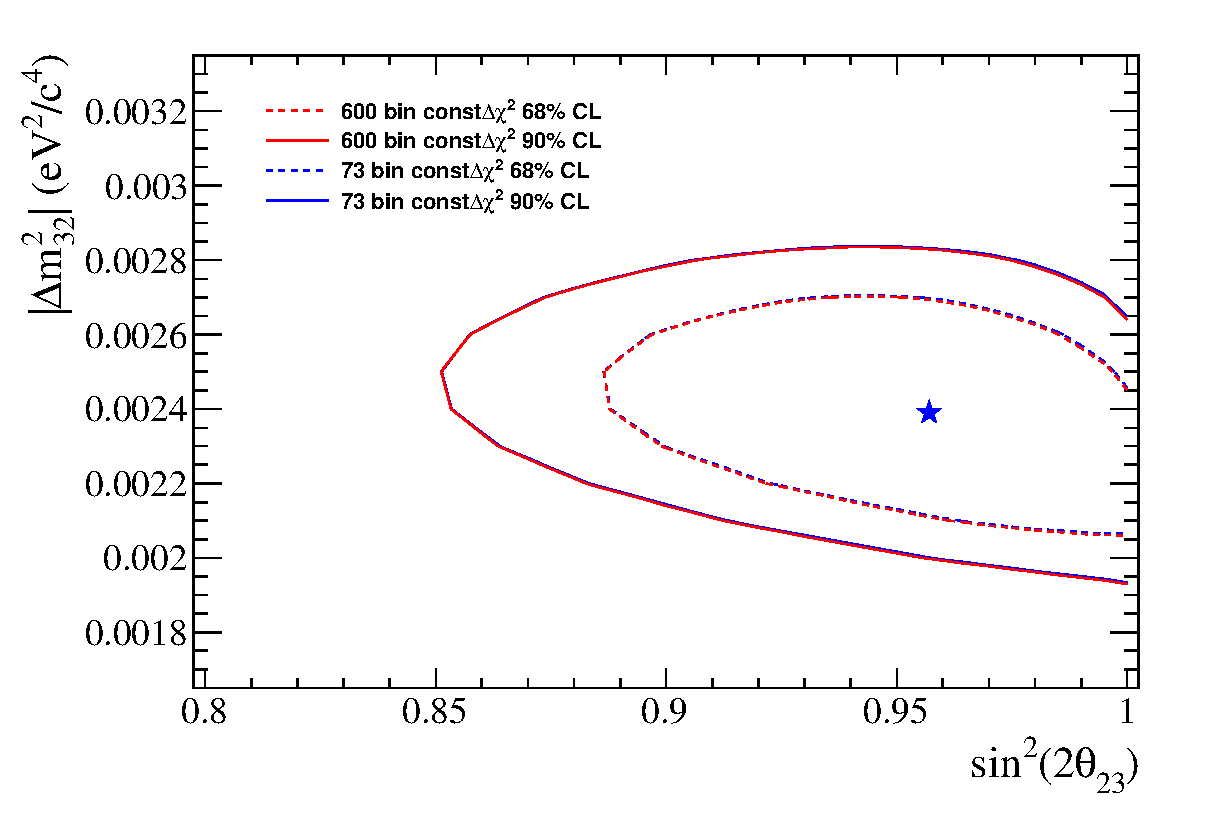
\includegraphics[width=25pc]{./images/sensitivities/2+8constdchisq/sensitivity_binning}
\caption {
  Sensitivity study using the 2+8 constant $\Delta \chi^2$ method. The 68\% and 90\% CL contours are shown.
  The input point is (sin$^22\theta_{23}$, $|\Delta m_{32}^2|$) =  (0.957, 0.00239 $eV^2/c^4$).
  The sensitivity has been calculated for both the \emph{normal} 73 $E_{reco}$ binning,
  as well as for 600 50 MeV bins from 0 - 30 GeV.}
\label{fig:apdx:bin:sensitivity:600vs73}
\end{figure*}

%
% ----------------------------------------
%

%
% Figs for \subsection{SuperK MC templates in the chosen binning}
%

\begin{figure*}[htb]
\center
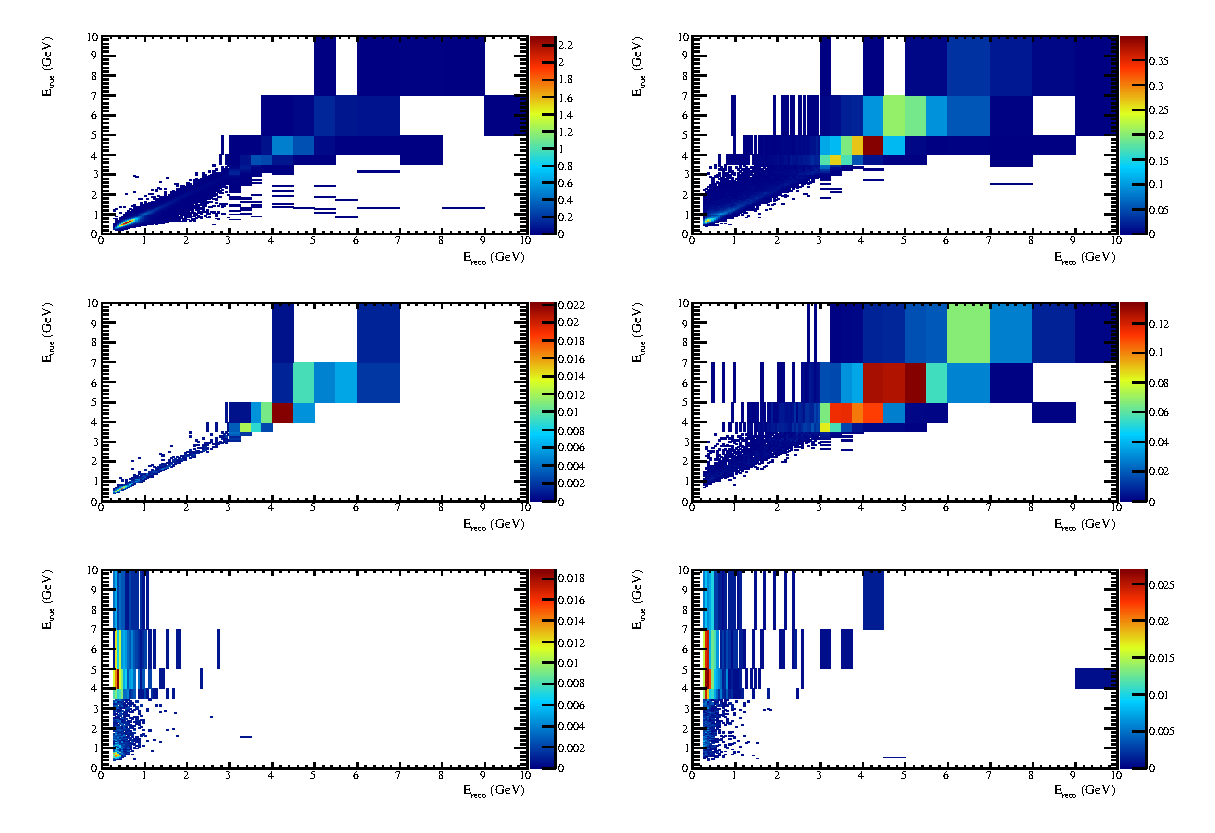
\includegraphics[width=35pc]{./images/spectrum_nominal/template_5}
\caption{
  Nominal ($E_{t}$, $E_{r}$) 1-ring $\mu$-like MC templates. 
  The templates are shown for
  $\nu_{\mu}$ CCQE (1)
  $\nu_{\mu}$ CC1$\pi$ (2), 
  $\nu_{\mu}$ CC coherent (3), 
  $\nu_{\mu}$ CC other (4), 
  $\nu_{\mu}$ NC1$\pi^{\pm}$ (5), 
  $\nu_{\mu}$ NC other (6).
}
\label{fig:etrue_ereco_templates:numu}
\end{figure*}

\begin{figure*}[htb]
\center
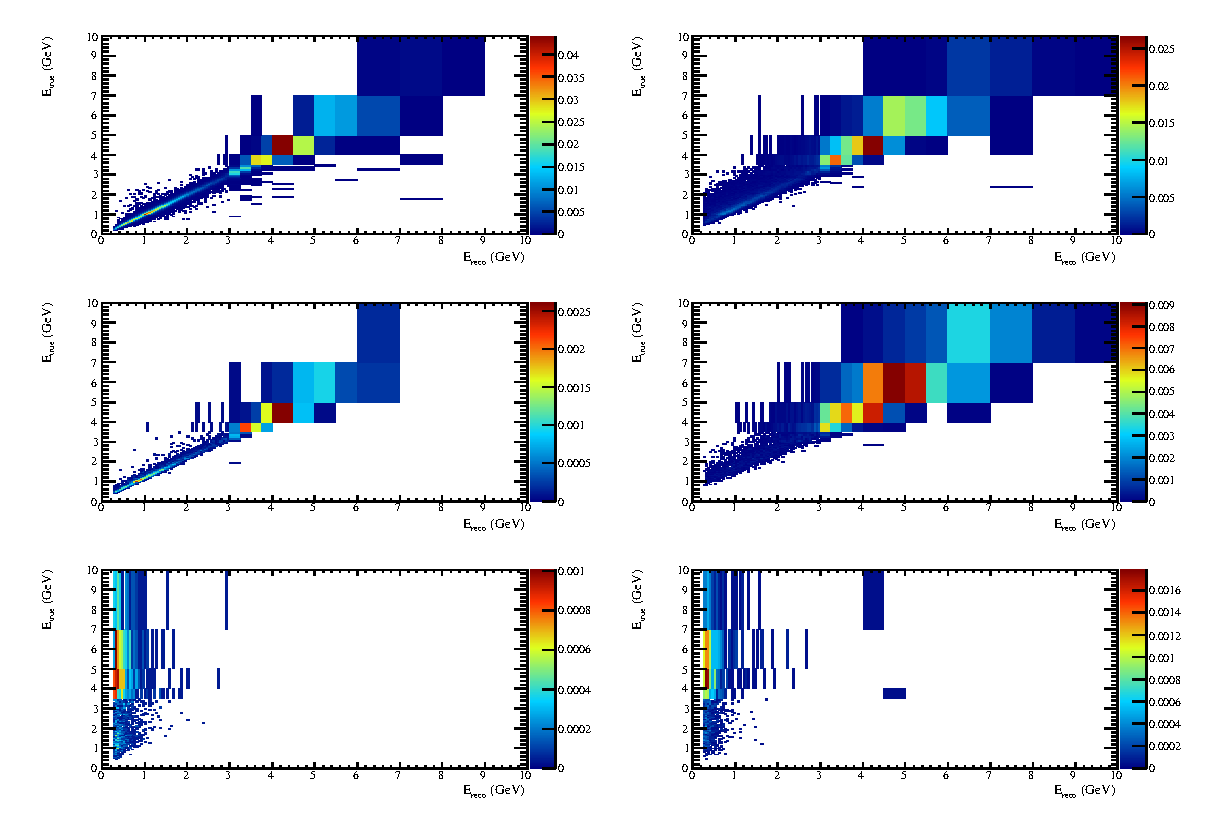
\includegraphics[width=35pc]{./images/spectrum_nominal/template_11}
\caption{
  Nominal ($E_{t}$, $E_{r}$) 1-ring $\mu$-like MC templates. 
  The templates are shown for
  $\bar{\nu_{\mu}}$ CCQE (7), 
  $\bar{\nu_{\mu}}$ CC1$\pi$ (8), 
  $\bar{\nu_{\mu}}$ CC coherent (9), 
  $\bar{\nu_{\mu}}$ CC other (10), 
  $\bar{\nu_{\mu}}$ NC1$\pi^{\pm}$ (11), 
  $\bar{\nu_{\mu}}$ NC other (12).
}
\label{fig:etrue_ereco_templates:numubar}
\end{figure*}

\begin{figure*}[htb]
\center
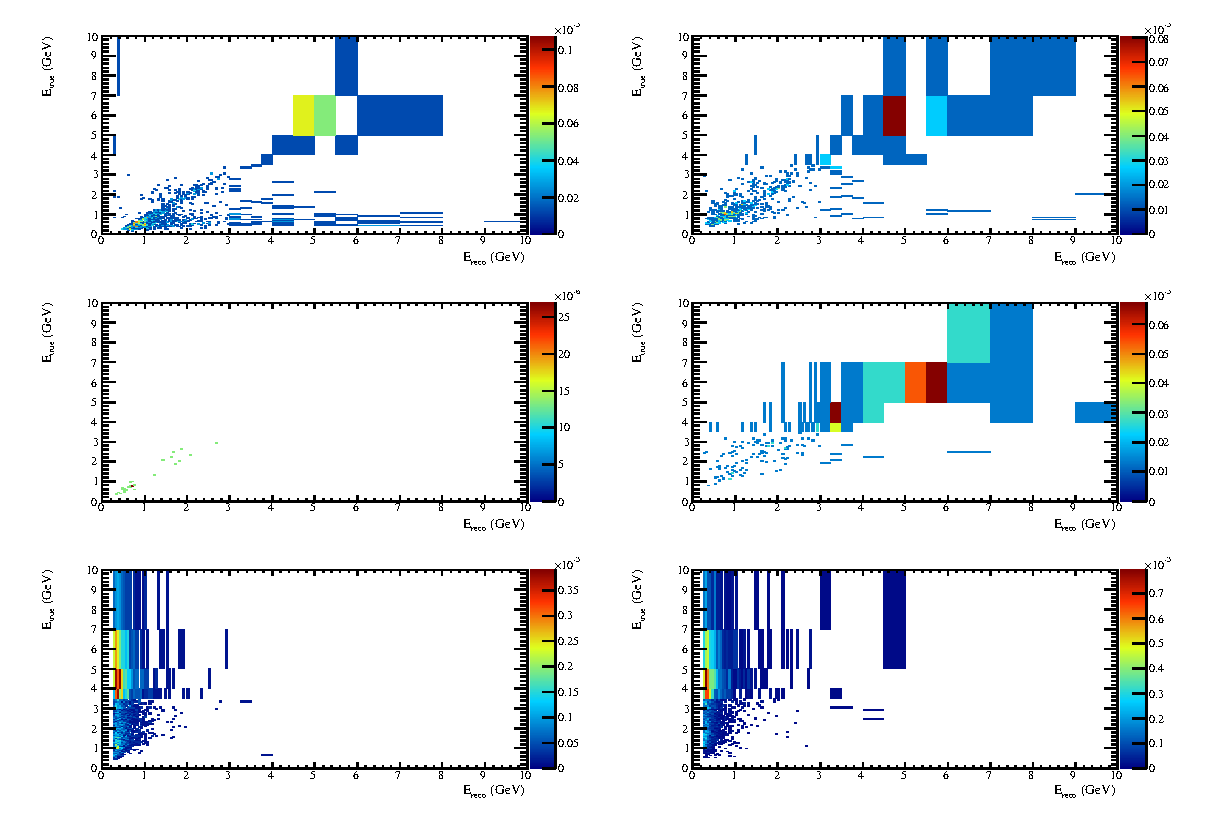
\includegraphics[width=35pc]{./images/spectrum_nominal/template_17}
\caption{
  Nominal ($E_{t}$, $E_{r}$) 1-ring $\mu$-like MC templates. 
  The templates are shown for
  $\nu_{e}$ CCQE (13), 
  $\nu_{e}$ CC1$\pi$ (14),
  $\nu_{e}$ CC coherent (15),
  $\nu_{e}$ CC other (16),
  $\nu_{e}$ NC1$\pi^{\pm}$ (17),
  $\nu_{e}$ NC other (18).
}
\label{fig:etrue_ereco_templates:nue}
\end{figure*}

\begin{figure*}[htb]
\center
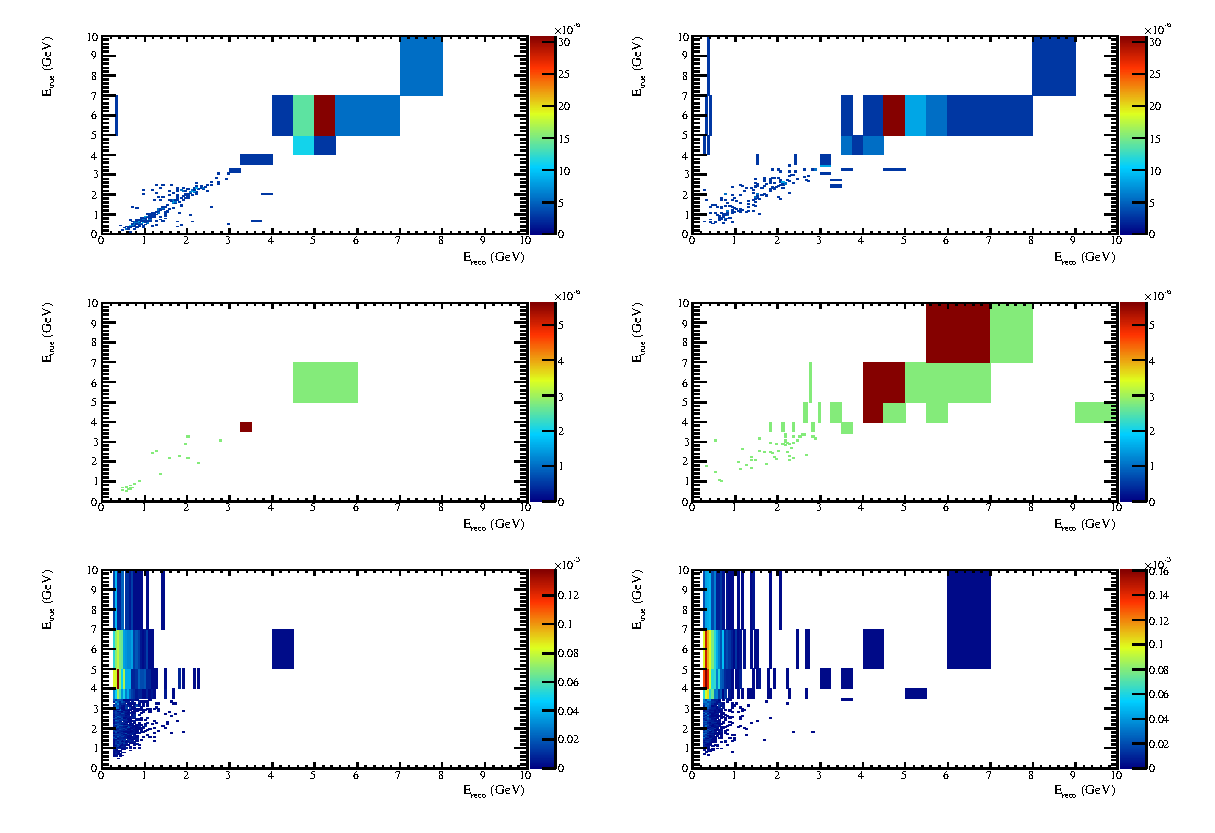
\includegraphics[width=35pc]{./images/spectrum_nominal/template_23}
\caption{
  Nominal ($E_{t}$, $E_{r}$) 1-ring $\mu$-like MC templates. 
  The templates are shown for
  $\bar{\nu_{e}}$ CCQE (19), 
  $\bar{\nu_{e}}$ CC1$\pi$ (20),
  $\bar{\nu_{e}}$ CC coherent (21),
  $\bar{\nu_{e}}$ CC other (22),
  $\bar{\nu_{e}}$ NC1$\pi^{\pm}$ (23),
  $\bar{\nu_{e}}$ NC other (24).
}
\label{fig:etrue_ereco_templates:nuebar}
\end{figure*}

\begin{figure*}[htb]
\center
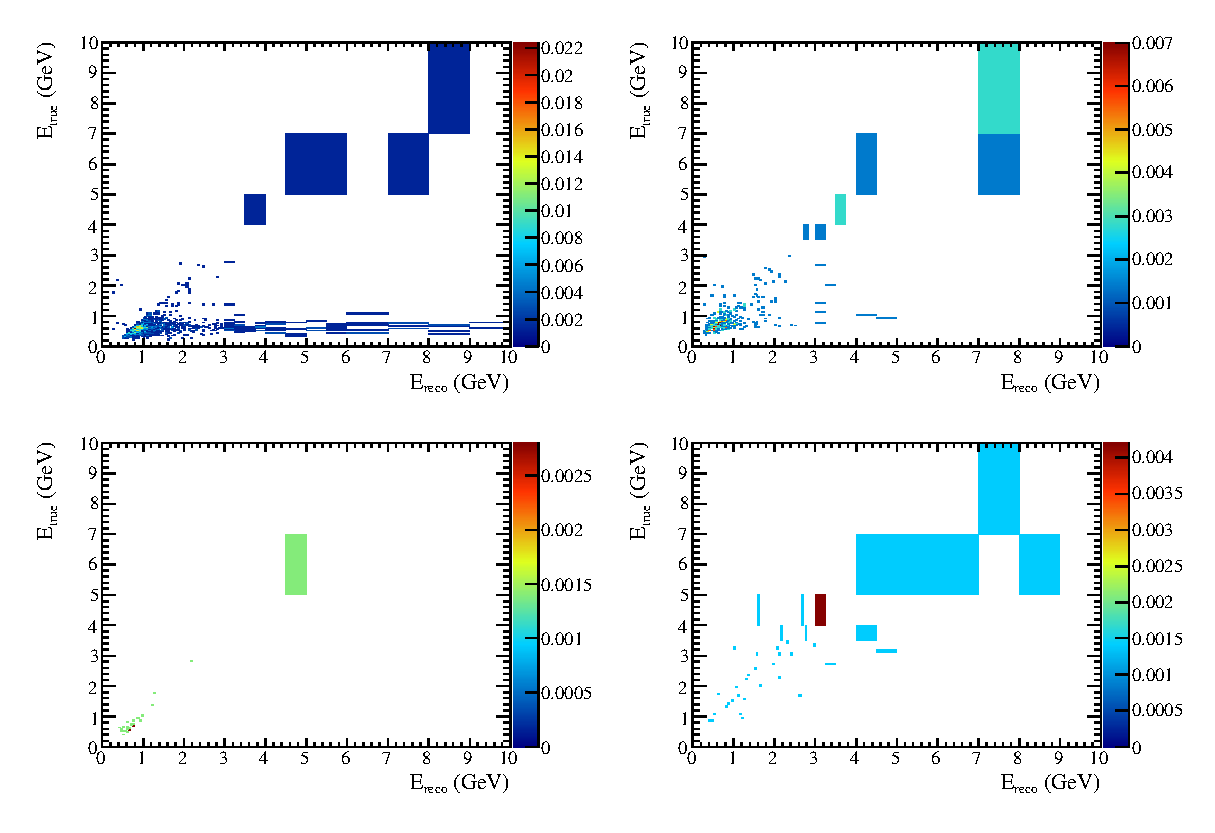
\includegraphics[width=35pc]{./images/spectrum_nominal/template_27}
\caption{
  Nominal ($E_{t}$, $E_{r}$) 1-ring $\mu$-like MC templates. 
  The templates are shown for
  osc. $\nu_{e}$ CCQE (25), 
  osc. $\nu_{e}$ CC1$\pi$ (26),
  osc. $\nu_{e}$ CC coherent (27) and
  osc. $\nu_{e}$ CC other (28).
}
\label{fig:etrue_ereco_templates:signue}
\end{figure*}


%
% ----------------------------------------
%

%
% Figs for \subsection{$E_{true}$ and $E_{reco}$ binning for systematic parameter response functions}
%

\begin{figure}[htb]
\center
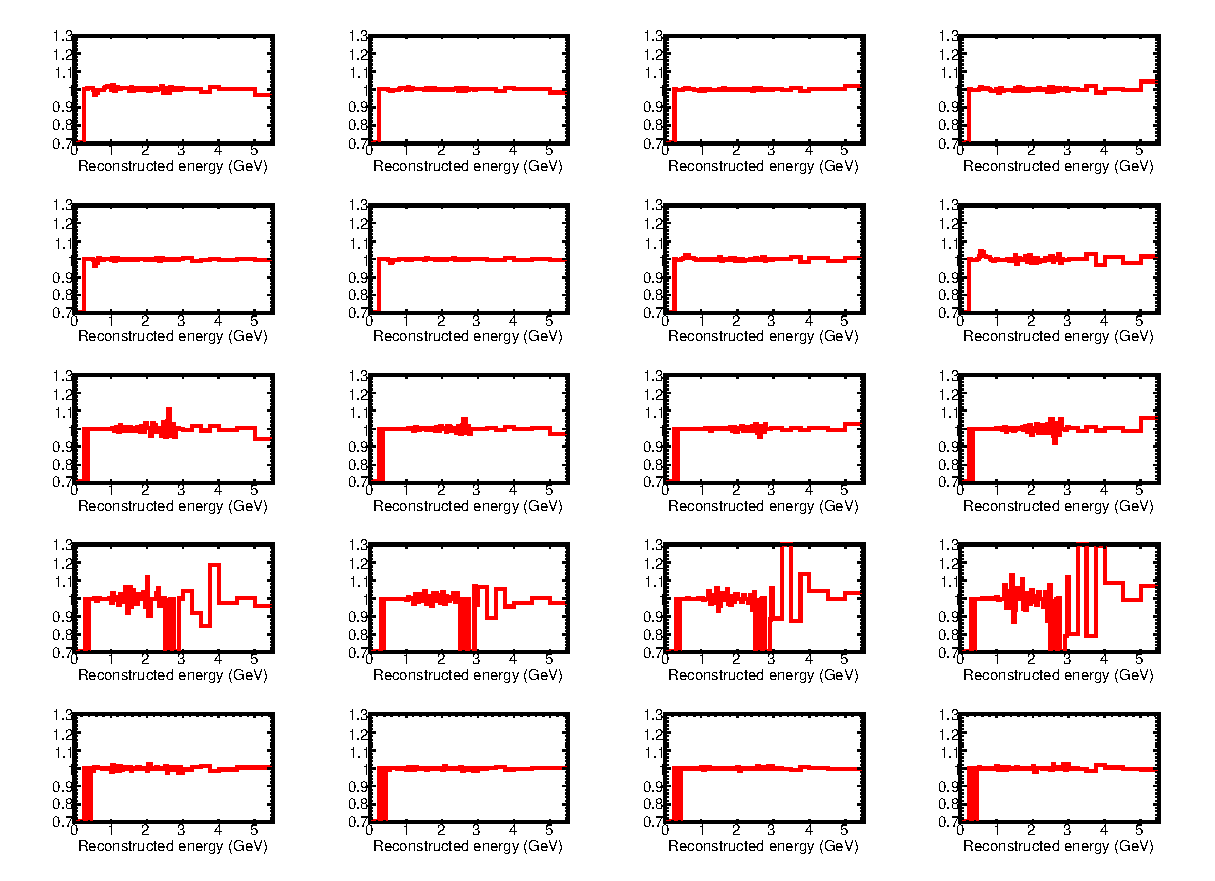
\includegraphics[width=40pc]{./images/spectrum_tweaked/MaQE}
\caption {
   Ratios of non-oscillated tweaked total SuperK MC E$_{reco}$ spectra made with the cross-section splines to those made with event-by-event reweighting 
   for MaQE. Each row represents one neutrino species, and these are $\nu_{\mu}$, $\bar{\nu}_{\mu}$, $\nu_{e}$ and $\bar{\nu}_{e}$ and oscillated $\nu_{e}$
   in that order. Each column represents a tweak value, and these are -2$\sigma$, -1$\sigma$, +1$\sigma$ and +2$\sigma$ in that order. Both the spline
   spectra and the event-by-event spectra are made with the 73-bin scheme given in Sec.\ \ref{sec:mc_templates:template_binning}.
}
\label{fig:spline_binning_studies:maqe}
\end{figure}

\begin{figure}[htb]
\center
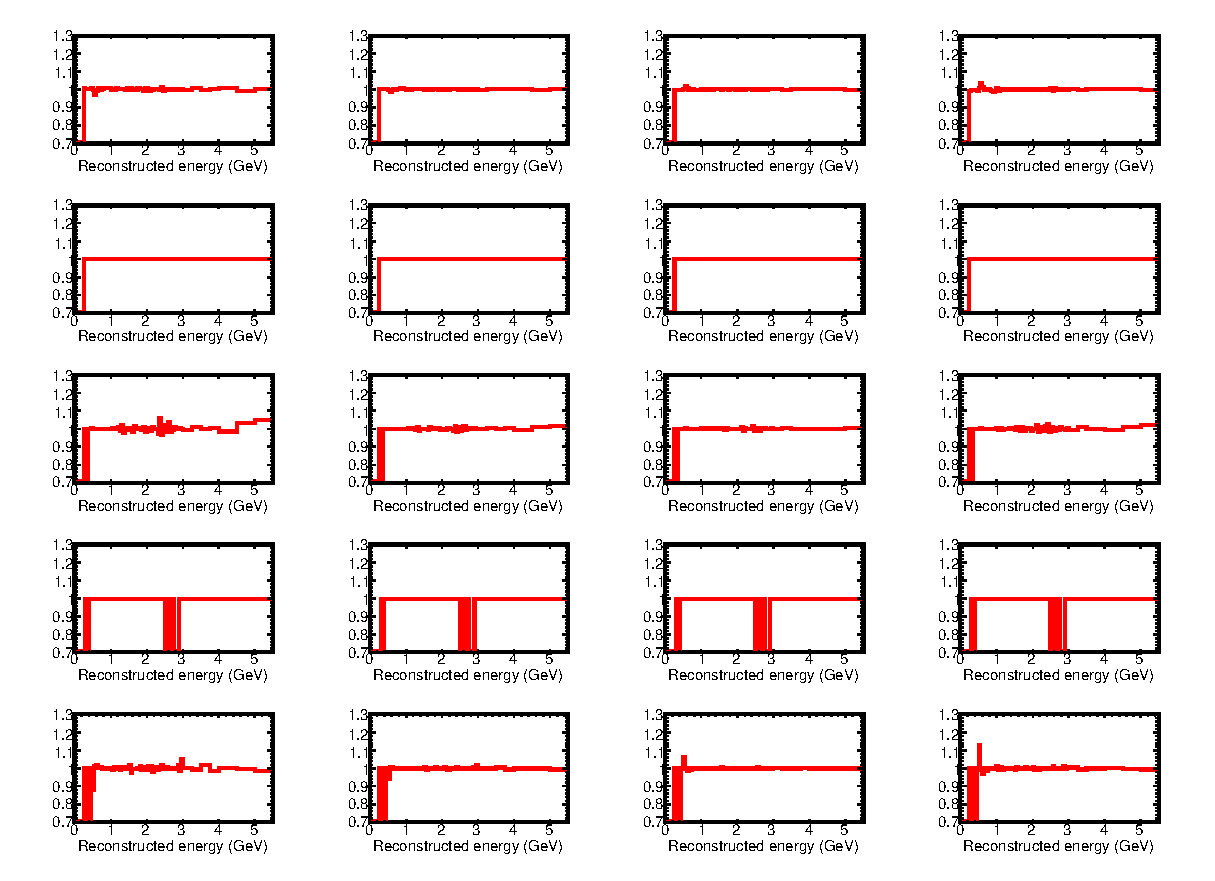
\includegraphics[width=40pc]{./images/spectrum_tweaked/pF}
\caption {
   Ratios of non-oscillated tweaked total SuperK MC E$_{reco}$ spectra made with the cross-section splines to those made with event-by-event reweighting 
   for the Fermi momentum.
   Each row represents one neutrino species, and these are $\nu_{\mu}$, $\bar{\nu}_{\mu}$, $\nu_{e}$ and $\bar{\nu}_{e}$ and oscillated $\nu_{e}$
   in that order. Each column represents a tweak value, and these are -2$\sigma$, -1$\sigma$, +1$\sigma$ and +2$\sigma$ in that order. Both the spline
   spectra and the event-by-event spectra are made with the 73-bin scheme given in Sec.\ \ref{sec:mc_templates:template_binning}.
}
\label{fig:spline_binning_studies:pf}
\end{figure}

\begin{figure}[htb]
\center
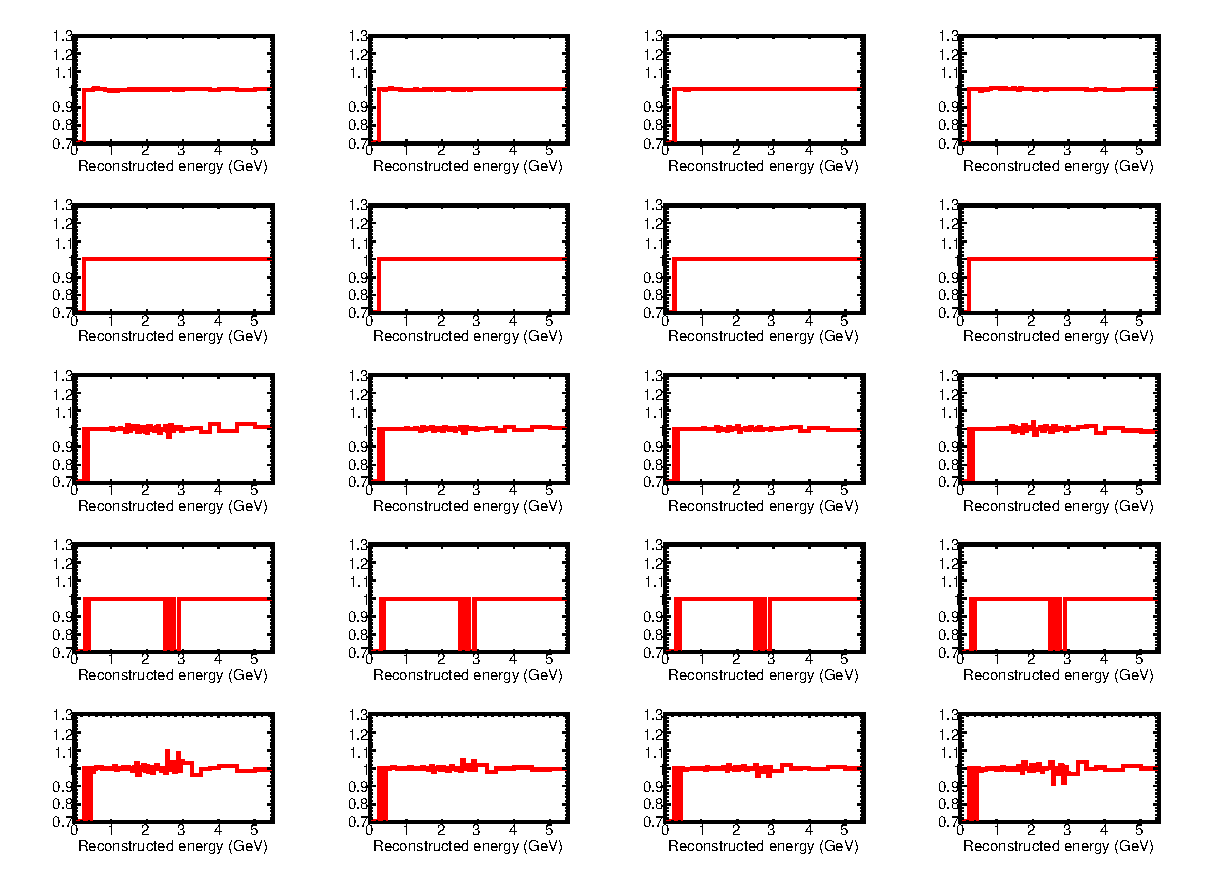
\includegraphics[width=40pc]{./images/spectrum_tweaked/BindE}
\caption {
   Ratios of non-oscillated tweaked total SuperK MC E$_{reco}$ spectra made with the cross-section splines to those made with event-by-event reweighting 
   for the binding energy.
   Each row represents one neutrino species, and these are $\nu_{\mu}$, $\bar{\nu}_{\mu}$, $\nu_{e}$ and $\bar{\nu}_{e}$ and oscillated $\nu_{e}$
   in that order. Each column represents a tweak value, and these are -2$\sigma$, -1$\sigma$, +1$\sigma$ and +2$\sigma$ in that order. Both the spline
   spectra and the event-by-event spectra are made with the 73-bin scheme given in Sec.\ \ref{sec:mc_templates:template_binning}.
}
\label{fig:spline_binning_studies:binde}
\end{figure}

\begin{figure}[htb]
\center
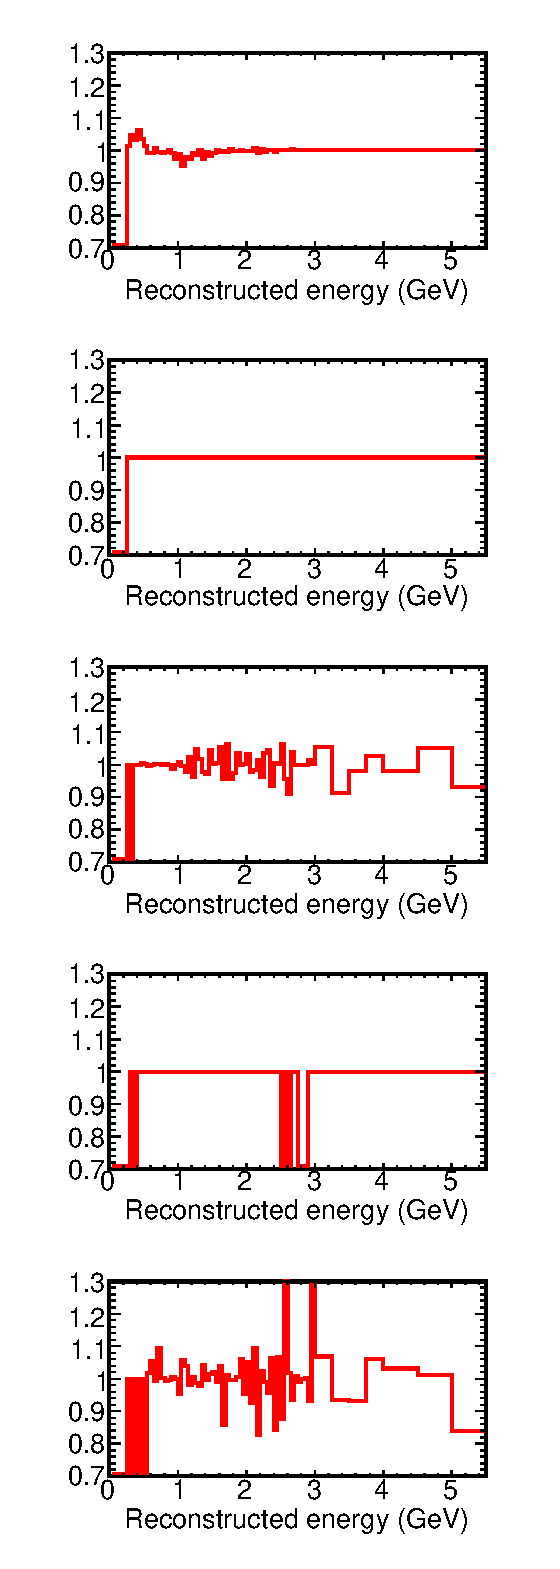
\includegraphics[width=10pc]{./images/spectrum_tweaked/SF}
\caption {
   Ratios of non-oscillated tweaked total SuperK MC E$_{reco}$ spectra made with the cross-section splines to those made with event-by-event reweighting 
   for the spectral function.
   Each histogram represents one neutrino species, and these are $\nu_{\mu}$, $\bar{\nu}_{\mu}$, $\nu_{e}$ and $\bar{\nu}_{e}$ and oscillated $\nu_{e}$
   in that order. Both the spline
   spectra and the event-by-event spectra are made with the 73-bin scheme given in Sec.\ \ref{sec:mc_templates:template_binning}.
}
\label{fig:spline_binning_studies:sf}
\end{figure}

\begin{figure}[htb]
\center
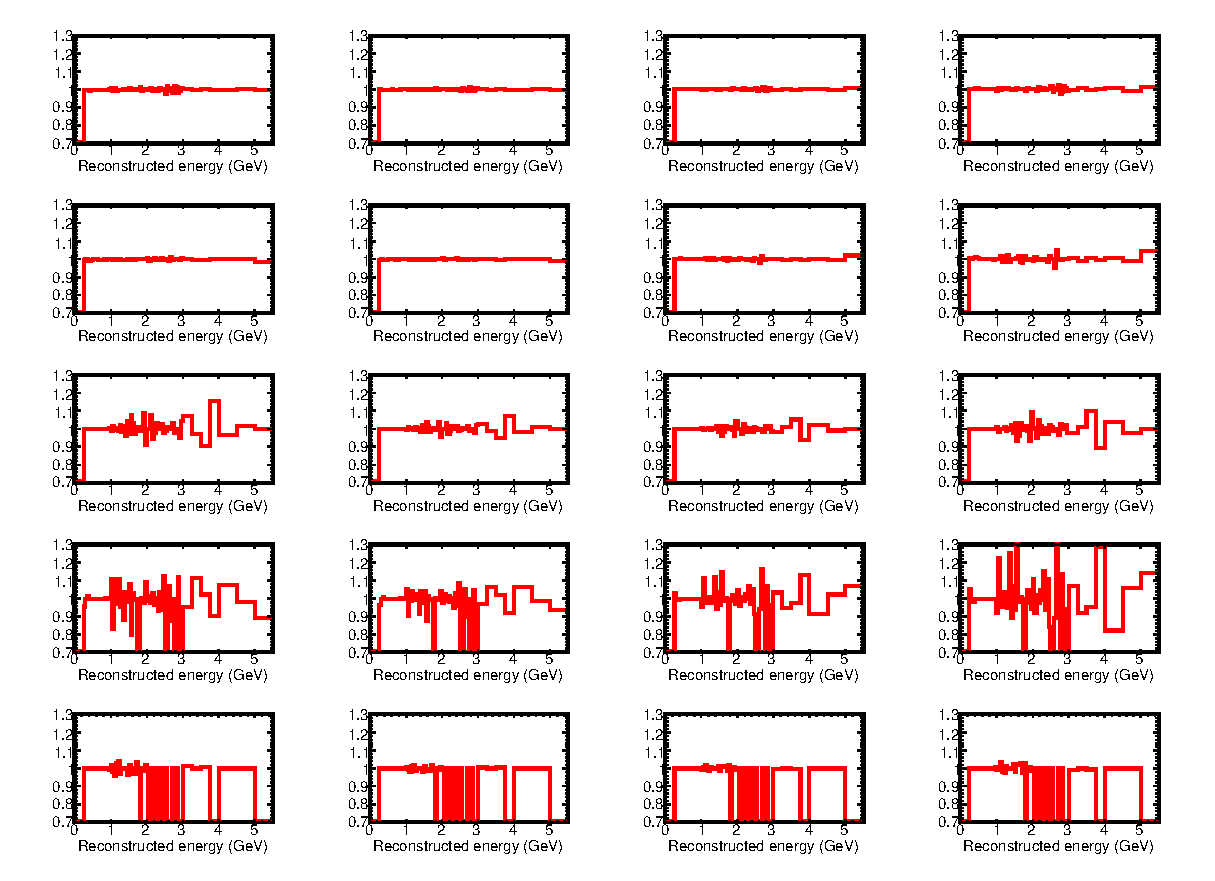
\includegraphics[width=40pc]{./images/spectrum_tweaked/MaResCC1pi}
\caption {
   Ratios of non-oscillated tweaked total SuperK MC E$_{reco}$ spectra made with the cross-section splines to those made with event-by-event reweighting 
   for MaRes for CC1$\pi$ interactions.
   Each row represents one neutrino species, and these are $\nu_{\mu}$, $\bar{\nu}_{\mu}$, $\nu_{e}$ and $\bar{\nu}_{e}$ and oscillated $\nu_{e}$
   in that order. Each column represents a tweak value, and these are -2$\sigma$, -1$\sigma$, +1$\sigma$ and +2$\sigma$ in that order. Both the spline
   spectra and the event-by-event spectra are made with the 73-bin scheme given in Sec.\ \ref{sec:mc_templates:template_binning}.
}
\label{fig:spline_binning_studies:mares}
\end{figure}

\begin{figure}[htb]
\center
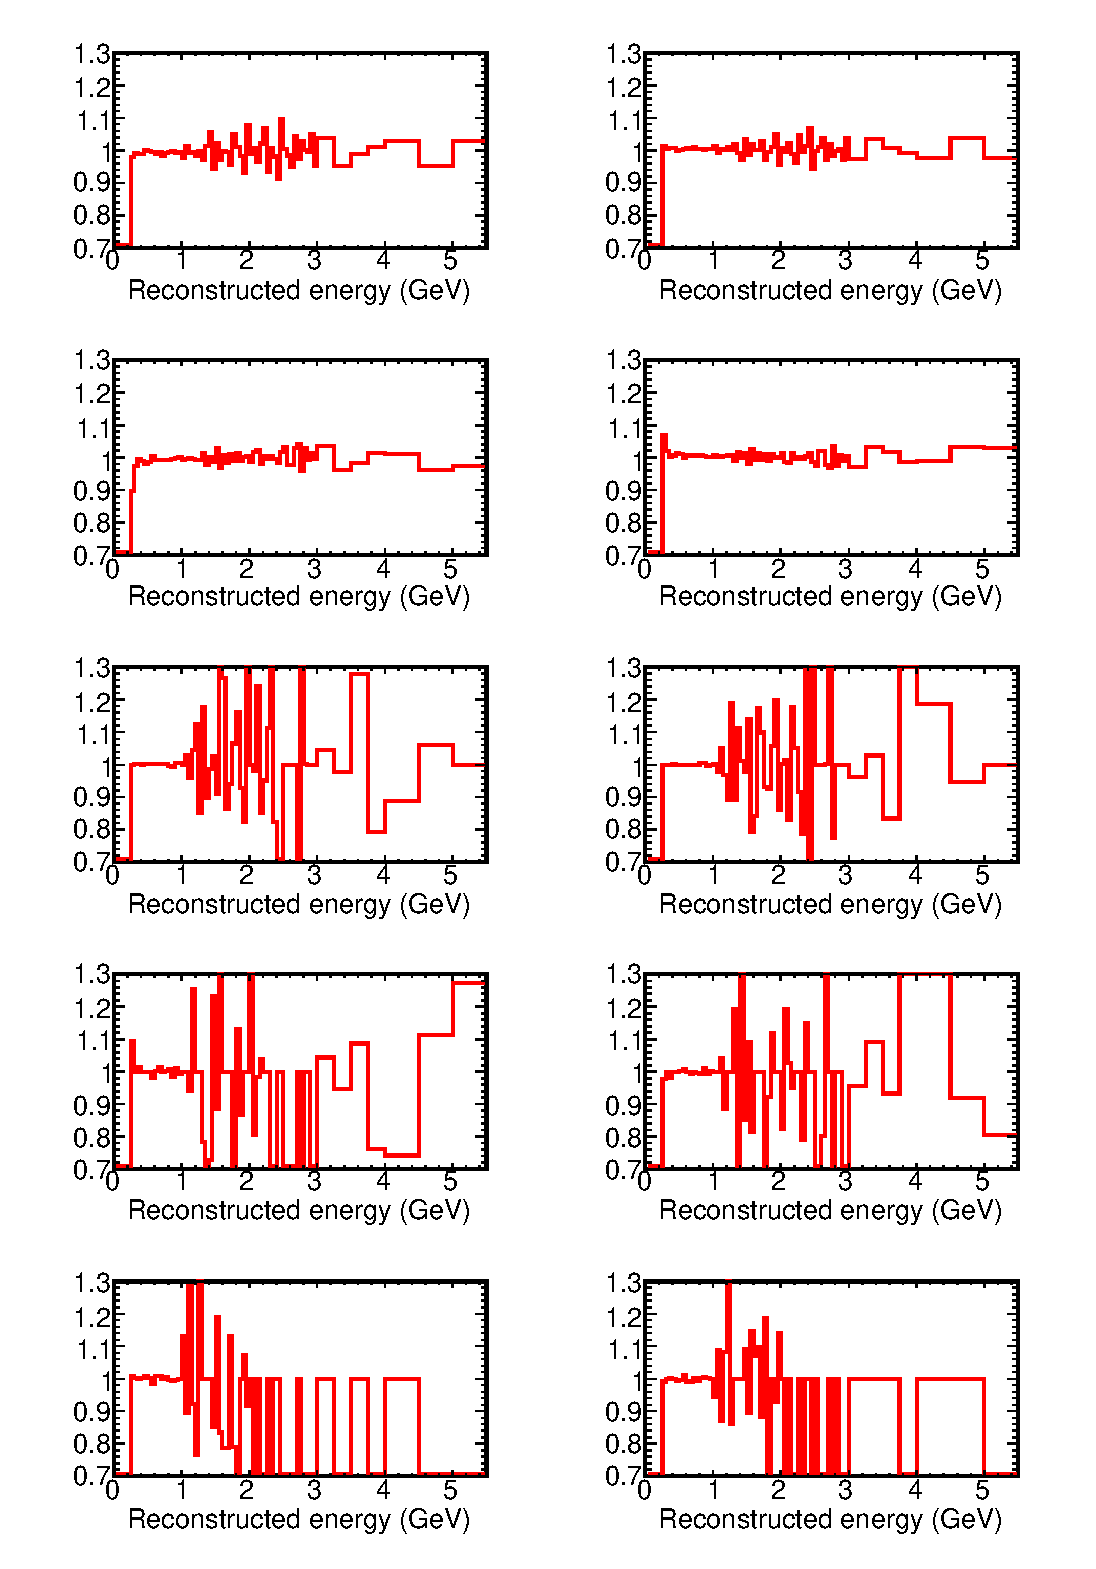
\includegraphics[width=20pc]{./images/spectrum_tweaked/PilessDeltaCC1pi}
\caption {
   Ratios of non-oscillated tweaked total SuperK MC E$_{reco}$ spectra made with the cross-section splines to those made with event-by-event reweighting 
   for the piless delta systematic for CC1$\pi$ interactions.
   Each row represents one neutrino species, and these are $\nu_{\mu}$, $\bar{\nu}_{\mu}$, $\nu_{e}$ and $\bar{\nu}_{e}$ and oscillated $\nu_{e}$
   in that order. Each column represents a tweak value, and these are -1$\sigma$, and +1$\sigma$ in that order. Both the spline
   spectra and the event-by-event spectra are made with the 73-bin scheme given in Sec.\ \ref{sec:mc_templates:template_binning}.
}
\label{fig:spline_binning_studies:pilessdelta}
\end{figure}

\begin{figure}[htb]
\center
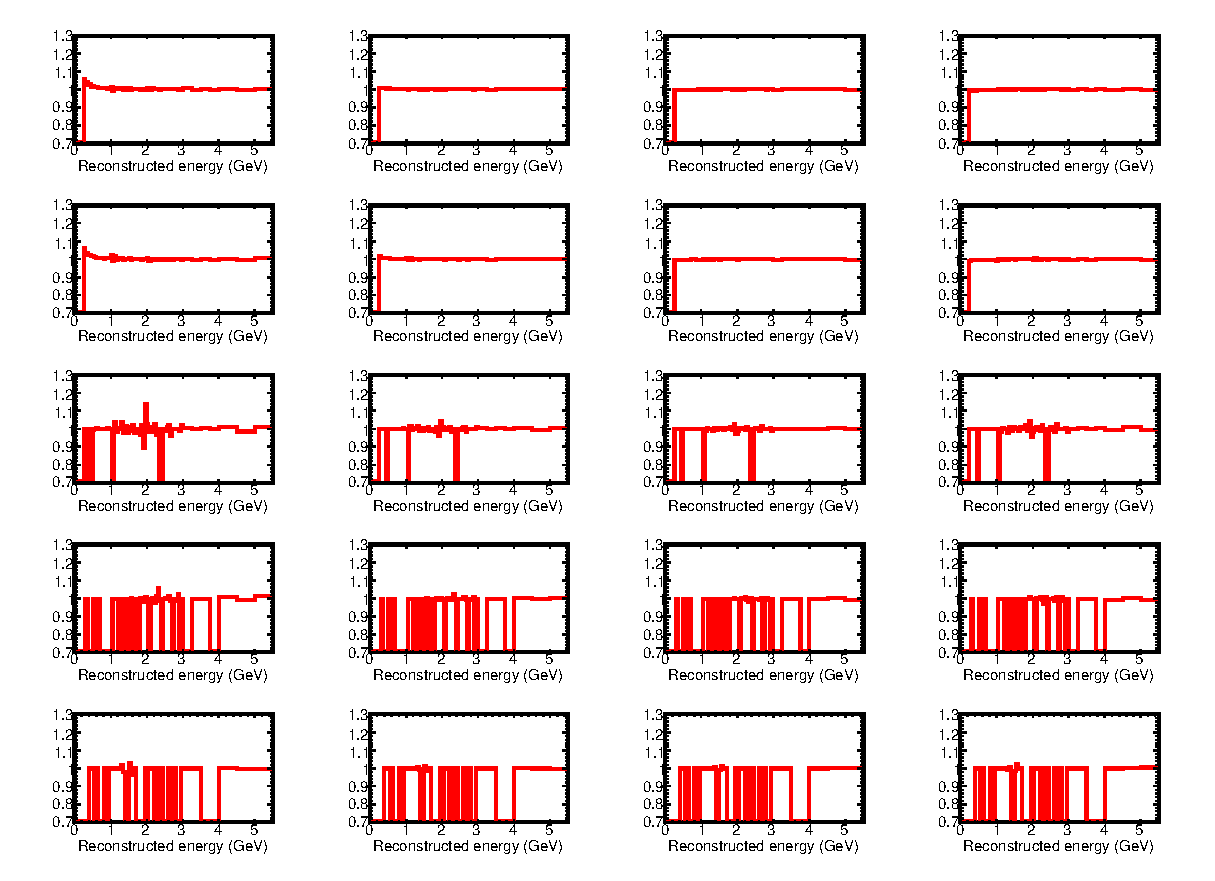
\includegraphics[width=40pc]{./images/spectrum_tweaked/CCotherShape}
\caption {
   Ratios of non-oscillated tweaked total SuperK MC E$_{reco}$ spectra made with the cross-section splines to those made with event-by-event reweighting 
   for the CC other shape systematic.  
   Each row represents one neutrino species, and these are $\nu_{\mu}$, $\bar{\nu}_{\mu}$, $\nu_{e}$ and $\bar{\nu}_{e}$ and oscillated $\nu_{e}$
   in that order. Each column represents a tweak value, and these are -2$\sigma$, -1$\sigma$, +1$\sigma$ and +2$\sigma$ in that order. Both the spline
   spectra and the event-by-event spectra are made with the 73-bin scheme given in Sec.\ \ref{sec:mc_templates:template_binning}.
}
\label{fig:spline_binning_studies:ccothershape}
\end{figure}

%
% ----------------------------------------
%
